\documentclass[landscape]{article}

\usepackage[utf8]{inputenc}
\usepackage[english]{babel}

\usepackage{amsmath,amsfonts,amssymb}
\usepackage{fullpage}
\usepackage{verbatim}

\usepackage[margin=10mm, top=10mm, bottom=5mm]{geometry}

\usepackage{tikz,pgfplots}

\pgfplotsset{
  width=240mm,height=190mm,
  major grid style={thin,dotted,color=black!50},
  minor grid style={thin,dotted,color=black!50},
  grid,
  every axis/.append style={
    line width=0.5pt,
    tick style={
      line cap=round,
      thin,
      major tick length=4pt,
      minor tick length=2pt,
    },
  },
  legend cell align=left,
  legend pos=north west,
  compat=1.9
}

%%%%%%%%%%%%%%%%%%%%%%%%%%%%%%%%%%%%%%%%%%%%%%%%%%%%%%%%%%%%%%%%%%%%%%%%%%%%%%%%

\begin{document}

% IMPORT-DATA ResultsQS ResultsQS_juqueen.txt

%%%%%%%%%%%%%%%%%%%%%%%%%%%%%%%%%%%%%%%%%%%%%%%%%%%%%%%%%%%%%%%%%%%%%%%%%%%%%%%%

\begin{center}

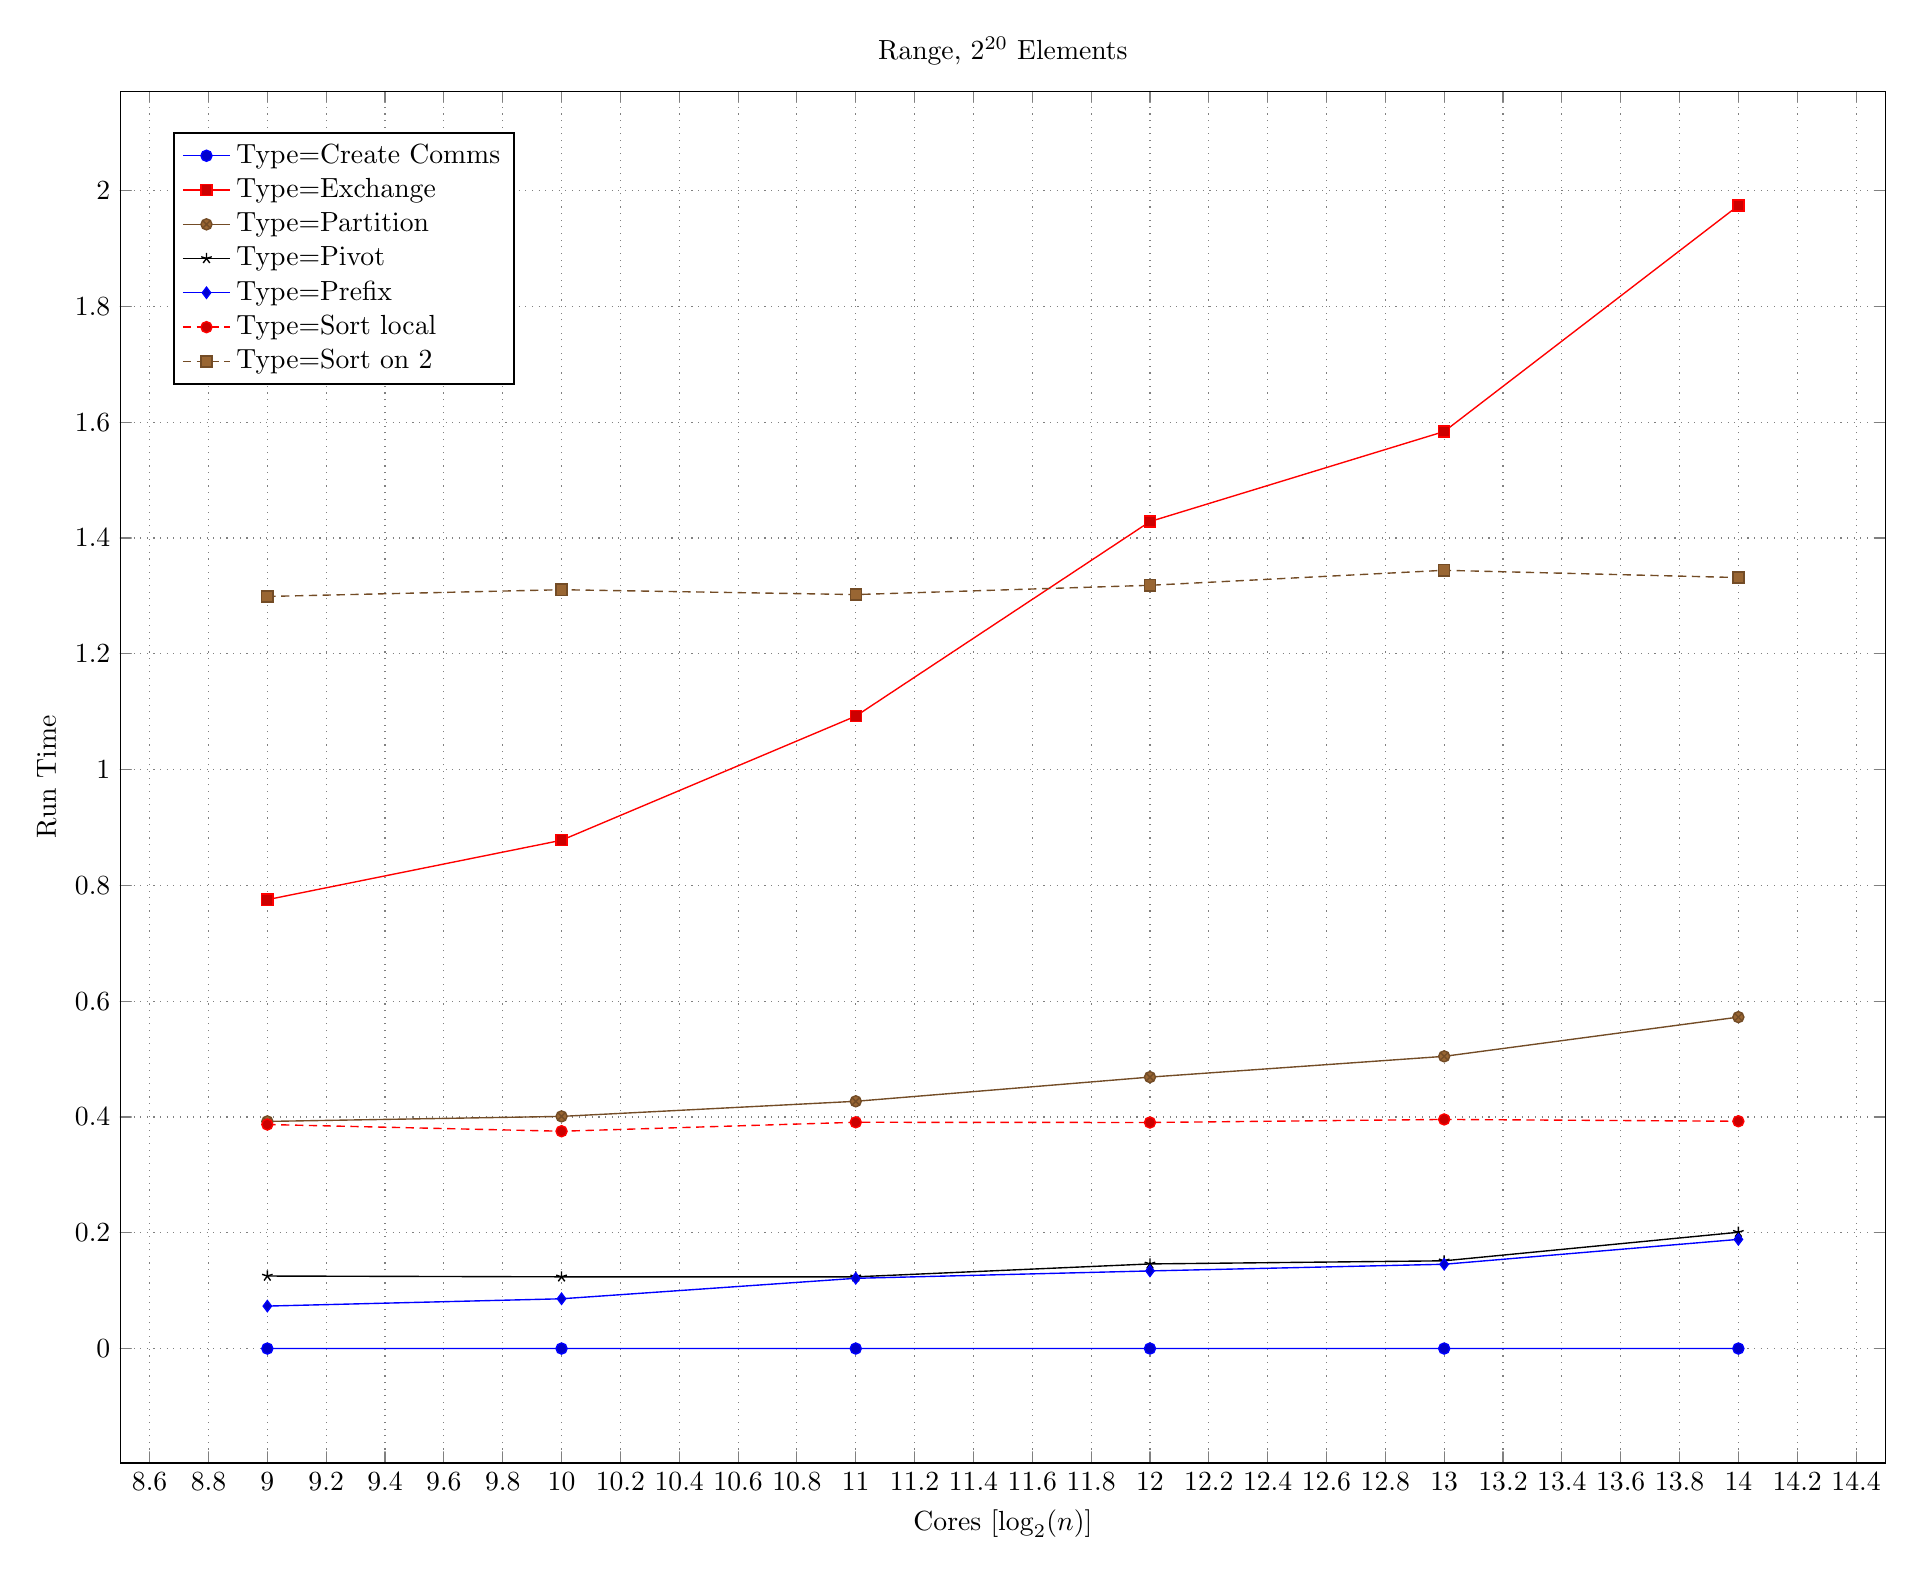
\begin{tikzpicture}
  \begin{axis}[
    title={Range, $2^{20}$ Elements},
    xlabel={Cores [$\log_2(n)$]},
    ylabel={Run Time},
    ]   
	%% MULTIPLOT(Type) SELECT elements, collective, LOG(2,size) AS x, Time as y, MULTIPLOT FROM (    
	%% SELECT elements, size, MEDIAN(pivot) as Time, 'Pivot' as Type, collective, blocking, mpi_split
	%% FROM ResultsQS
	%% GROUP BY collective, size, elements, blocking, mpi_split
	%% UNION ALL
	%% SELECT elements, size, MEDIAN(partition) as Time, 'Partition' as Type, collective, blocking, mpi_split
	%% FROM ResultsQS
	%% GROUP BY collective, size, elements, blocking, mpi_split
	%% UNION ALL
	%% SELECT elements, size, MEDIAN(calculate) as Time, 'Prefix' as Type, collective, blocking, mpi_split
	%% FROM ResultsQS
	%% GROUP BY collective, size, elements, blocking, mpi_split
	%% UNION ALL
	%% SELECT elements, size, MEDIAN(exchange) as Time, 'Exchange' as Type, collective, blocking, mpi_split
	%% FROM ResultsQS
	%% GROUP BY collective, size, elements, blocking, mpi_split
	%% UNION ALL
	%% SELECT elements, size, MEDIAN(create_comms) as Time, 'Create Comms' as Type, collective, blocking, mpi_split
	%% FROM ResultsQS
	%% GROUP BY collective, size, elements, blocking, mpi_split
	%% UNION ALL
	%% SELECT elements, size, MEDIAN(sort_two) as Time, 'Sort on 2' as Type, collective, blocking, mpi_split
	%% FROM ResultsQS
	%% GROUP BY collective, size, elements, blocking, mpi_split
	%% UNION ALL
	%% SELECT elements, size, MEDIAN(sort_local) as Time, 'Sort local' as Type, collective, blocking, mpi_split
	%% FROM ResultsQS
	%% GROUP BY collective, size, elements, blocking, mpi_split
	%% ) a
	%% WHERE collective="range" AND elements=POWER(2,20) AND blocking=0 AND mpi_split=0
	%% GROUP BY MULTIPLOT, x  ORDER BY MULTIPLOT, x
 \addplot coordinates { (9.0,2.91787e-05) (10.0,3.09069e-05) (11.0,3.31669e-05) (12.0,3.76519e-05) (13.0,4.19431e-05) (14.0,4.578e-05) };
 \addlegendentry{Type=Create Comms};
 \addplot coordinates { (9.0,0.775366) (10.0,0.877971) (11.0,1.09236) (12.0,1.42844) (13.0,1.58398) (14.0,1.97417) };
 \addlegendentry{Type=Exchange};
 \addplot coordinates { (9.0,0.392331) (10.0,0.401033) (11.0,0.427104) (12.0,0.468899) (13.0,0.504746) (14.0,0.572511) };
 \addlegendentry{Type=Partition};
 \addplot coordinates { (9.0,0.125294) (10.0,0.123921) (11.0,0.123916) (12.0,0.146194) (13.0,0.151579) (14.0,0.200895) };
 \addlegendentry{Type=Pivot};
 \addplot coordinates { (9.0,0.0733838) (10.0,0.0860003) (11.0,0.121367) (12.0,0.134109) (13.0,0.145614) (14.0,0.188622) };
 \addlegendentry{Type=Prefix};
 \addplot coordinates { (9.0,0.387005) (10.0,0.375397) (11.0,0.390876) (12.0,0.390506) (13.0,0.395763) (14.0,0.392627) };
 \addlegendentry{Type=Sort local};
 \addplot coordinates { (9.0,1.29907) (10.0,1.31072) (11.0,1.30234) (12.0,1.31836) (13.0,1.34426) (14.0,1.33172) };
 \addlegendentry{Type=Sort on 2};


  \end{axis}
\end{tikzpicture}
\newpage

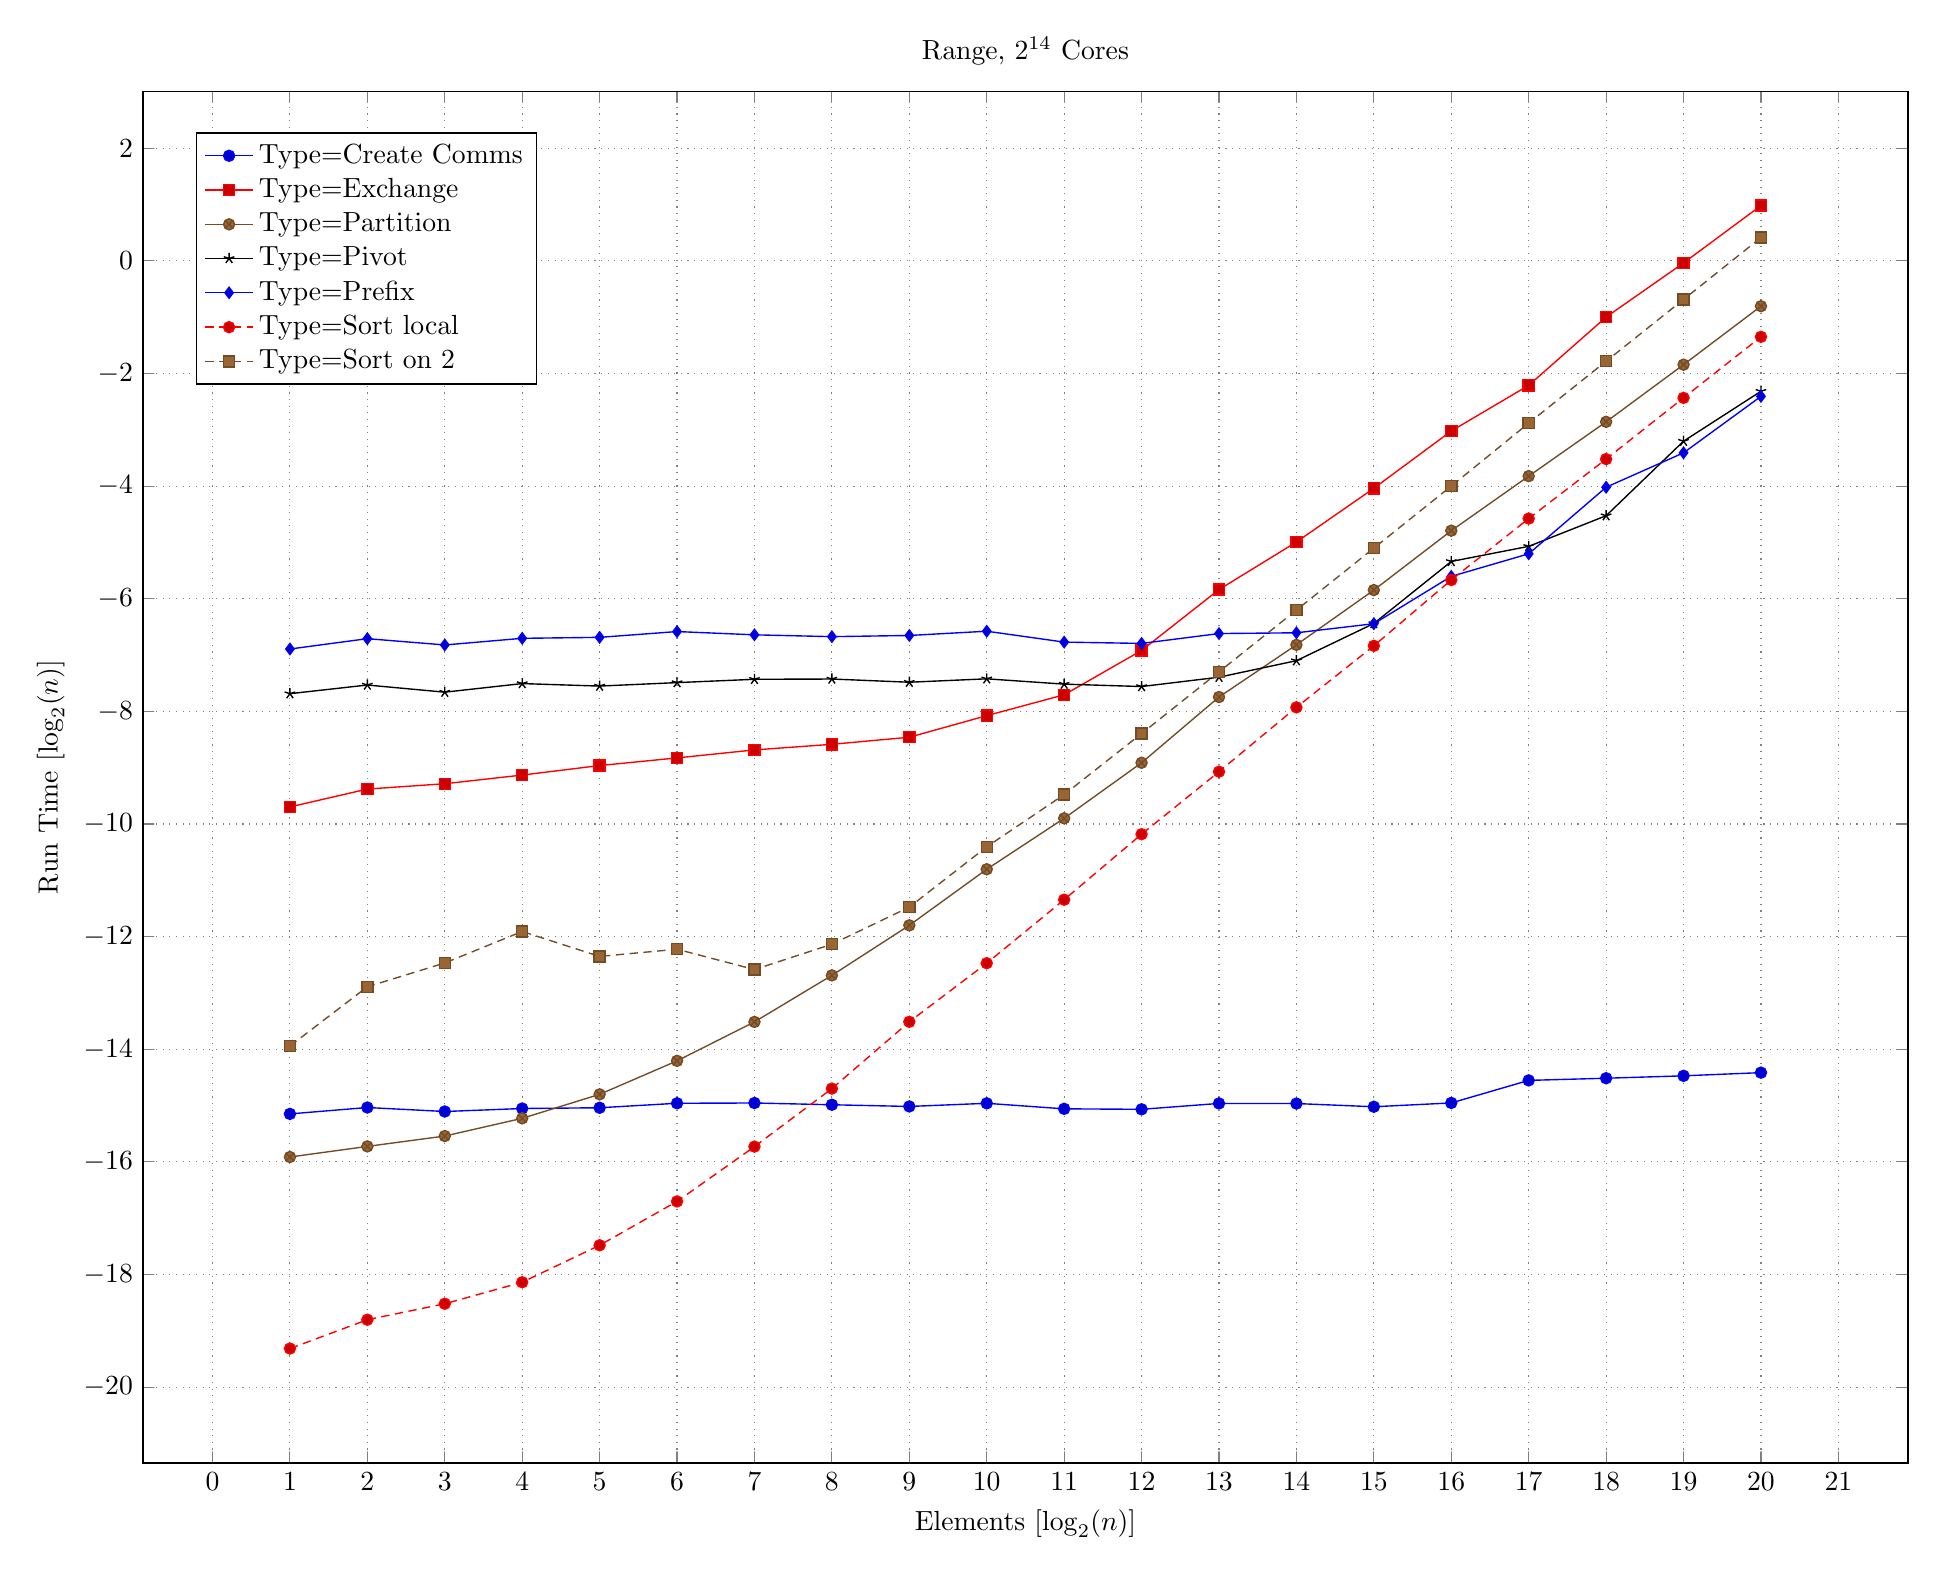
\begin{tikzpicture}
\begin{axis}[
title={Range, $2^{14}$ Cores},
xlabel={Elements [$\log_2(n)$]},
ylabel={Run Time [$\log_2(n)$]},
]   
%% MULTIPLOT(Type) SELECT size, collective, LOG(2,elements) AS x, LOG(2,Time) as y, MULTIPLOT FROM (    
%% SELECT elements, size, MEDIAN(pivot) as Time, 'Pivot' as Type, collective, blocking, mpi_split
%% FROM ResultsQS
%% GROUP BY collective, size, elements, blocking, mpi_split
%% UNION ALL
%% SELECT elements, size, MEDIAN(partition) as Time, 'Partition' as Type, collective, blocking, mpi_split
%% FROM ResultsQS
%% GROUP BY collective, size, elements, blocking, mpi_split
%% UNION ALL
%% SELECT elements, size, MEDIAN(calculate) as Time, 'Prefix' as Type, collective, blocking, mpi_split
%% FROM ResultsQS
%% GROUP BY collective, size, elements, blocking, mpi_split
%% UNION ALL
%% SELECT elements, size, MEDIAN(exchange) as Time, 'Exchange' as Type, collective, blocking, mpi_split
%% FROM ResultsQS
%% GROUP BY collective, size, elements, blocking, mpi_split
%% UNION ALL
%% SELECT elements, size, MEDIAN(create_comms) as Time, 'Create Comms' as Type, collective, blocking, mpi_split
%% FROM ResultsQS
%% GROUP BY collective, size, elements, blocking, mpi_split
%% UNION ALL
%% SELECT elements, size, MEDIAN(sort_two) as Time, 'Sort on 2' as Type, collective, blocking, mpi_split
%% FROM ResultsQS
%% GROUP BY collective, size, elements, blocking, mpi_split
%% UNION ALL
%% SELECT elements, size, MEDIAN(sort_local) as Time, 'Sort local' as Type, collective, blocking, mpi_split
%% FROM ResultsQS
%% GROUP BY collective, size, elements, blocking, mpi_split
%% ) a
%% WHERE collective="range" AND size=16384 AND blocking=0 AND mpi_split=0
%% GROUP BY MULTIPLOT, x  ORDER BY MULTIPLOT, x
\addplot coordinates { (1.0,-15.1477) (2.0,-15.0343) (3.0,-15.1051) (4.0,-15.0521) (5.0,-15.0385) (6.0,-14.959) (7.0,-14.954) (8.0,-14.9854) (9.0,-15.0155) (10.0,-14.9596) (11.0,-15.0578) (12.0,-15.0661) (13.0,-14.9618) (14.0,-14.9639) (15.0,-15.0207) (16.0,-14.9531) (17.0,-14.5526) (18.0,-14.5142) (19.0,-14.4716) (20.0,-14.4149) };
\addlegendentry{Type=Create Comms};
\addplot coordinates { (1.0,-9.69649) (2.0,-9.37933) (3.0,-9.28483) (4.0,-9.13069) (5.0,-8.96194) (6.0,-8.8263) (7.0,-8.68412) (8.0,-8.58467) (9.0,-8.45901) (10.0,-8.07598) (11.0,-7.70507) (12.0,-6.91789) (13.0,-5.83694) (14.0,-4.99241) (15.0,-4.03856) (16.0,-3.0217) (17.0,-2.21026) (18.0,-0.998227) (19.0,-0.0369506) (20.0,0.981246) };
\addlegendentry{Type=Exchange};
\addplot coordinates { (1.0,-15.9131) (2.0,-15.7249) (3.0,-15.541) (4.0,-15.2261) (5.0,-14.8003) (6.0,-14.2057) (7.0,-13.5141) (8.0,-12.6878) (9.0,-11.7991) (10.0,-10.8034) (11.0,-9.89936) (12.0,-8.91235) (13.0,-7.7449) (14.0,-6.81826) (15.0,-5.84586) (16.0,-4.79133) (17.0,-3.82267) (18.0,-2.85841) (19.0,-1.84337) (20.0,-0.804625) };
\addlegendentry{Type=Partition};
\addplot coordinates { (1.0,-7.68558) (2.0,-7.53205) (3.0,-7.65904) (4.0,-7.50634) (5.0,-7.55067) (6.0,-7.48916) (7.0,-7.43024) (8.0,-7.42538) (9.0,-7.48241) (10.0,-7.42186) (11.0,-7.51623) (12.0,-7.55886) (13.0,-7.39294) (14.0,-7.09985) (15.0,-6.43929) (16.0,-5.33773) (17.0,-5.06951) (18.0,-4.52556) (19.0,-3.20205) (20.0,-2.31549) };
\addlegendentry{Type=Pivot};
\addplot coordinates { (1.0,-6.89255) (2.0,-6.7087) (3.0,-6.82056) (4.0,-6.70262) (5.0,-6.68529) (6.0,-6.58259) (7.0,-6.64051) (8.0,-6.6729) (9.0,-6.65215) (10.0,-6.57644) (11.0,-6.7698) (12.0,-6.79324) (13.0,-6.61798) (14.0,-6.60455) (15.0,-6.44319) (16.0,-5.60284) (17.0,-5.20216) (18.0,-4.01986) (19.0,-3.40869) (20.0,-2.40643) };
\addlegendentry{Type=Prefix};
\addplot coordinates { (1.0,-19.3145) (2.0,-18.8027) (3.0,-18.5191) (4.0,-18.1372) (5.0,-17.4804) (6.0,-16.7019) (7.0,-15.7286) (8.0,-14.6981) (9.0,-13.5127) (10.0,-12.4715) (11.0,-11.3441) (12.0,-10.1809) (13.0,-9.07075) (14.0,-7.92822) (15.0,-6.83586) (16.0,-5.66683) (17.0,-4.57604) (18.0,-3.51968) (19.0,-2.43235) (20.0,-1.34877) };
\addlegendentry{Type=Sort local};
\addplot coordinates { (1.0,-13.9433) (2.0,-12.8898) (3.0,-12.4679) (4.0,-11.9086) (5.0,-12.3512) (6.0,-12.2238) (7.0,-12.5845) (8.0,-12.1349) (9.0,-11.4757) (10.0,-10.4052) (11.0,-9.47687) (12.0,-8.39349) (13.0,-7.29842) (14.0,-6.20102) (15.0,-5.10064) (16.0,-3.99968) (17.0,-2.88165) (18.0,-1.78229) (19.0,-0.685457) (20.0,0.413291) };
\addlegendentry{Type=Sort on 2};


\end{axis}
\end{tikzpicture}
\newpage

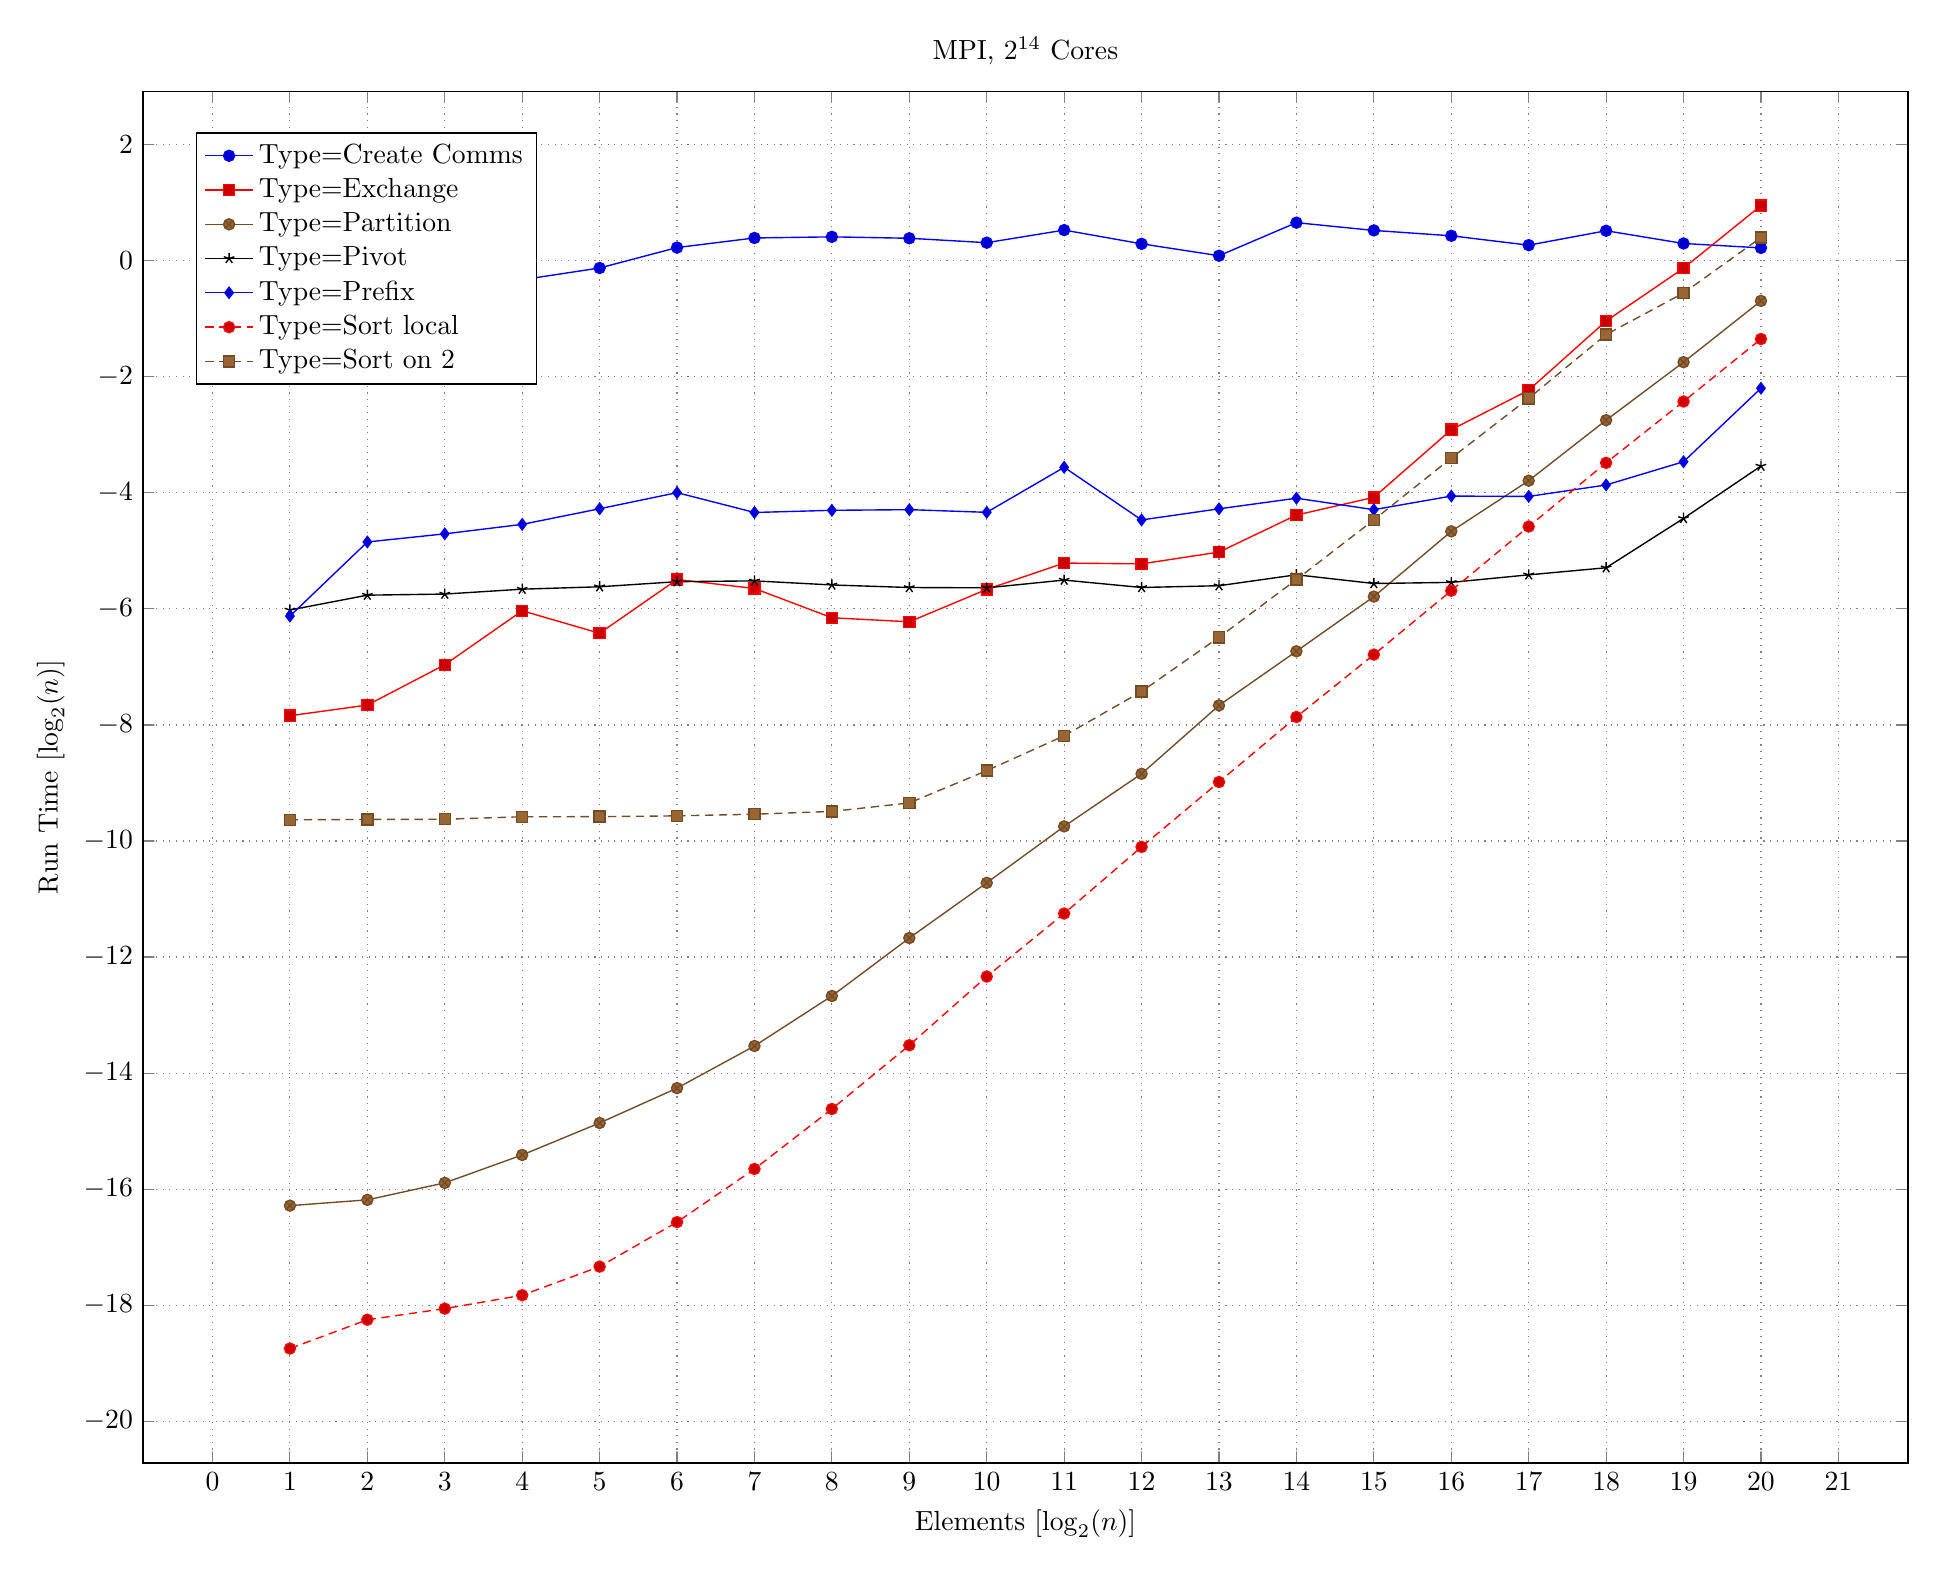
\begin{tikzpicture}
  \begin{axis}[
    title={MPI, $2^{14}$ Cores},
    xlabel={Elements [$\log_2(n)$]},
    ylabel={Run Time [$\log_2(n)$]},
    ]   
	%% MULTIPLOT(Type) SELECT size, collective, LOG(2,elements) AS x, LOG(2,Time) as y, MULTIPLOT FROM (    
	%% SELECT elements, size, MEDIAN(pivot) as Time, 'Pivot' as Type, collective, blocking, mpi_split
	%% FROM ResultsQS
	%% GROUP BY collective, size, elements, blocking, mpi_split
	%% UNION ALL
	%% SELECT elements, size, MEDIAN(partition) as Time, 'Partition' as Type, collective, blocking, mpi_split
	%% FROM ResultsQS
	%% GROUP BY collective, size, elements, blocking, mpi_split
	%% UNION ALL
	%% SELECT elements, size, MEDIAN(calculate) as Time, 'Prefix' as Type, collective, blocking, mpi_split
	%% FROM ResultsQS
	%% GROUP BY collective, size, elements, blocking, mpi_split
	%% UNION ALL
	%% SELECT elements, size, MEDIAN(exchange) as Time, 'Exchange' as Type, collective, blocking, mpi_split
	%% FROM ResultsQS
	%% GROUP BY collective, size, elements, blocking, mpi_split
	%% UNION ALL
	%% SELECT elements, size, MEDIAN(create_comms) as Time, 'Create Comms' as Type, collective, blocking, mpi_split
	%% FROM ResultsQS
	%% GROUP BY collective, size, elements, blocking, mpi_split
	%% UNION ALL
	%% SELECT elements, size, MEDIAN(sort_two) as Time, 'Sort on 2' as Type, collective, blocking, mpi_split
	%% FROM ResultsQS
	%% GROUP BY collective, size, elements, blocking, mpi_split
	%% UNION ALL
	%% SELECT elements, size, MEDIAN(sort_local) as Time, 'Sort local' as Type, collective, blocking, mpi_split
	%% FROM ResultsQS
	%% GROUP BY collective, size, elements, blocking, mpi_split
	%% ) a
	%% WHERE collective="mpi" AND size=16384 AND blocking=1 AND mpi_split=1
	%% GROUP BY MULTIPLOT, x  ORDER BY MULTIPLOT, x
 \addplot coordinates { (1.0,-1.37211) (2.0,-0.876191) (3.0,-0.689453) (4.0,-0.326682) (5.0,-0.124429) (6.0,0.227877) (7.0,0.393218) (8.0,0.412565) (9.0,0.387936) (10.0,0.311829) (11.0,0.529111) (12.0,0.292417) (13.0,0.0871641) (14.0,0.657036) (15.0,0.52298) (16.0,0.430767) (17.0,0.269033) (18.0,0.51779) (19.0,0.297954) (20.0,0.222533) };
 \addlegendentry{Type=Create Comms};
 \addplot coordinates { (1.0,-7.84059) (2.0,-7.6577) (3.0,-6.96242) (4.0,-6.03227) (5.0,-6.41974) (6.0,-5.49282) (7.0,-5.64784) (8.0,-6.15266) (9.0,-6.22217) (10.0,-5.66323) (11.0,-5.20967) (12.0,-5.22385) (13.0,-5.02046) (14.0,-4.38262) (15.0,-4.07716) (16.0,-2.91162) (17.0,-2.23017) (18.0,-1.0382) (19.0,-0.127512) (20.0,0.950901) };
 \addlegendentry{Type=Exchange};
 \addplot coordinates { (1.0,-16.2846) (2.0,-16.1851) (3.0,-15.8925) (4.0,-15.4113) (5.0,-14.8599) (6.0,-14.2593) (7.0,-13.533) (8.0,-12.6713) (9.0,-11.6724) (10.0,-10.7208) (11.0,-9.74838) (12.0,-8.84144) (13.0,-7.66282) (14.0,-6.72996) (15.0,-5.78752) (16.0,-4.66355) (17.0,-3.78984) (18.0,-2.74695) (19.0,-1.74741) (20.0,-0.69156) };
 \addlegendentry{Type=Partition};
 \addplot coordinates { (1.0,-6.01912) (2.0,-5.76319) (3.0,-5.74401) (4.0,-5.65991) (5.0,-5.61858) (6.0,-5.53065) (7.0,-5.51684) (8.0,-5.5872) (9.0,-5.63117) (10.0,-5.6368) (11.0,-5.50319) (12.0,-5.63084) (13.0,-5.6004) (14.0,-5.41155) (15.0,-5.56241) (16.0,-5.54273) (17.0,-5.41284) (18.0,-5.2907) (19.0,-4.44045) (20.0,-3.53796) };
 \addlegendentry{Type=Pivot};
 \addplot coordinates { (1.0,-6.12401) (2.0,-4.8465) (3.0,-4.7063) (4.0,-4.54297) (5.0,-4.27367) (6.0,-3.99638) (7.0,-4.33802) (8.0,-4.30077) (9.0,-4.28939) (10.0,-4.33546) (11.0,-3.55909) (12.0,-4.46659) (13.0,-4.27498) (14.0,-4.09211) (15.0,-4.28959) (16.0,-4.05555) (17.0,-4.06144) (18.0,-3.86403) (19.0,-3.46307) (20.0,-2.19705) };
 \addlegendentry{Type=Prefix};
 \addplot coordinates { (1.0,-18.7477) (2.0,-18.2512) (3.0,-18.06) (4.0,-17.8287) (5.0,-17.3357) (6.0,-16.5684) (7.0,-15.653) (8.0,-14.6191) (9.0,-13.5203) (10.0,-12.336) (11.0,-11.2499) (12.0,-10.1016) (13.0,-8.98351) (14.0,-7.86292) (15.0,-6.78737) (16.0,-5.68634) (17.0,-4.58005) (18.0,-3.48251) (19.0,-2.42511) (20.0,-1.34808) };
 \addlegendentry{Type=Sort local};
 \addplot coordinates { (1.0,-9.6343) (2.0,-9.62878) (3.0,-9.62554) (4.0,-9.5822) (5.0,-9.58051) (6.0,-9.56666) (7.0,-9.53834) (8.0,-9.49023) (9.0,-9.34421) (10.0,-8.78753) (11.0,-8.18696) (12.0,-7.4228) (13.0,-6.48944) (14.0,-5.49504) (15.0,-4.4658) (16.0,-3.40058) (17.0,-2.37) (18.0,-1.27125) (19.0,-0.555846) (20.0,0.400724) };
 \addlegendentry{Type=Sort on 2};


  \end{axis}
\end{tikzpicture}
\newpage

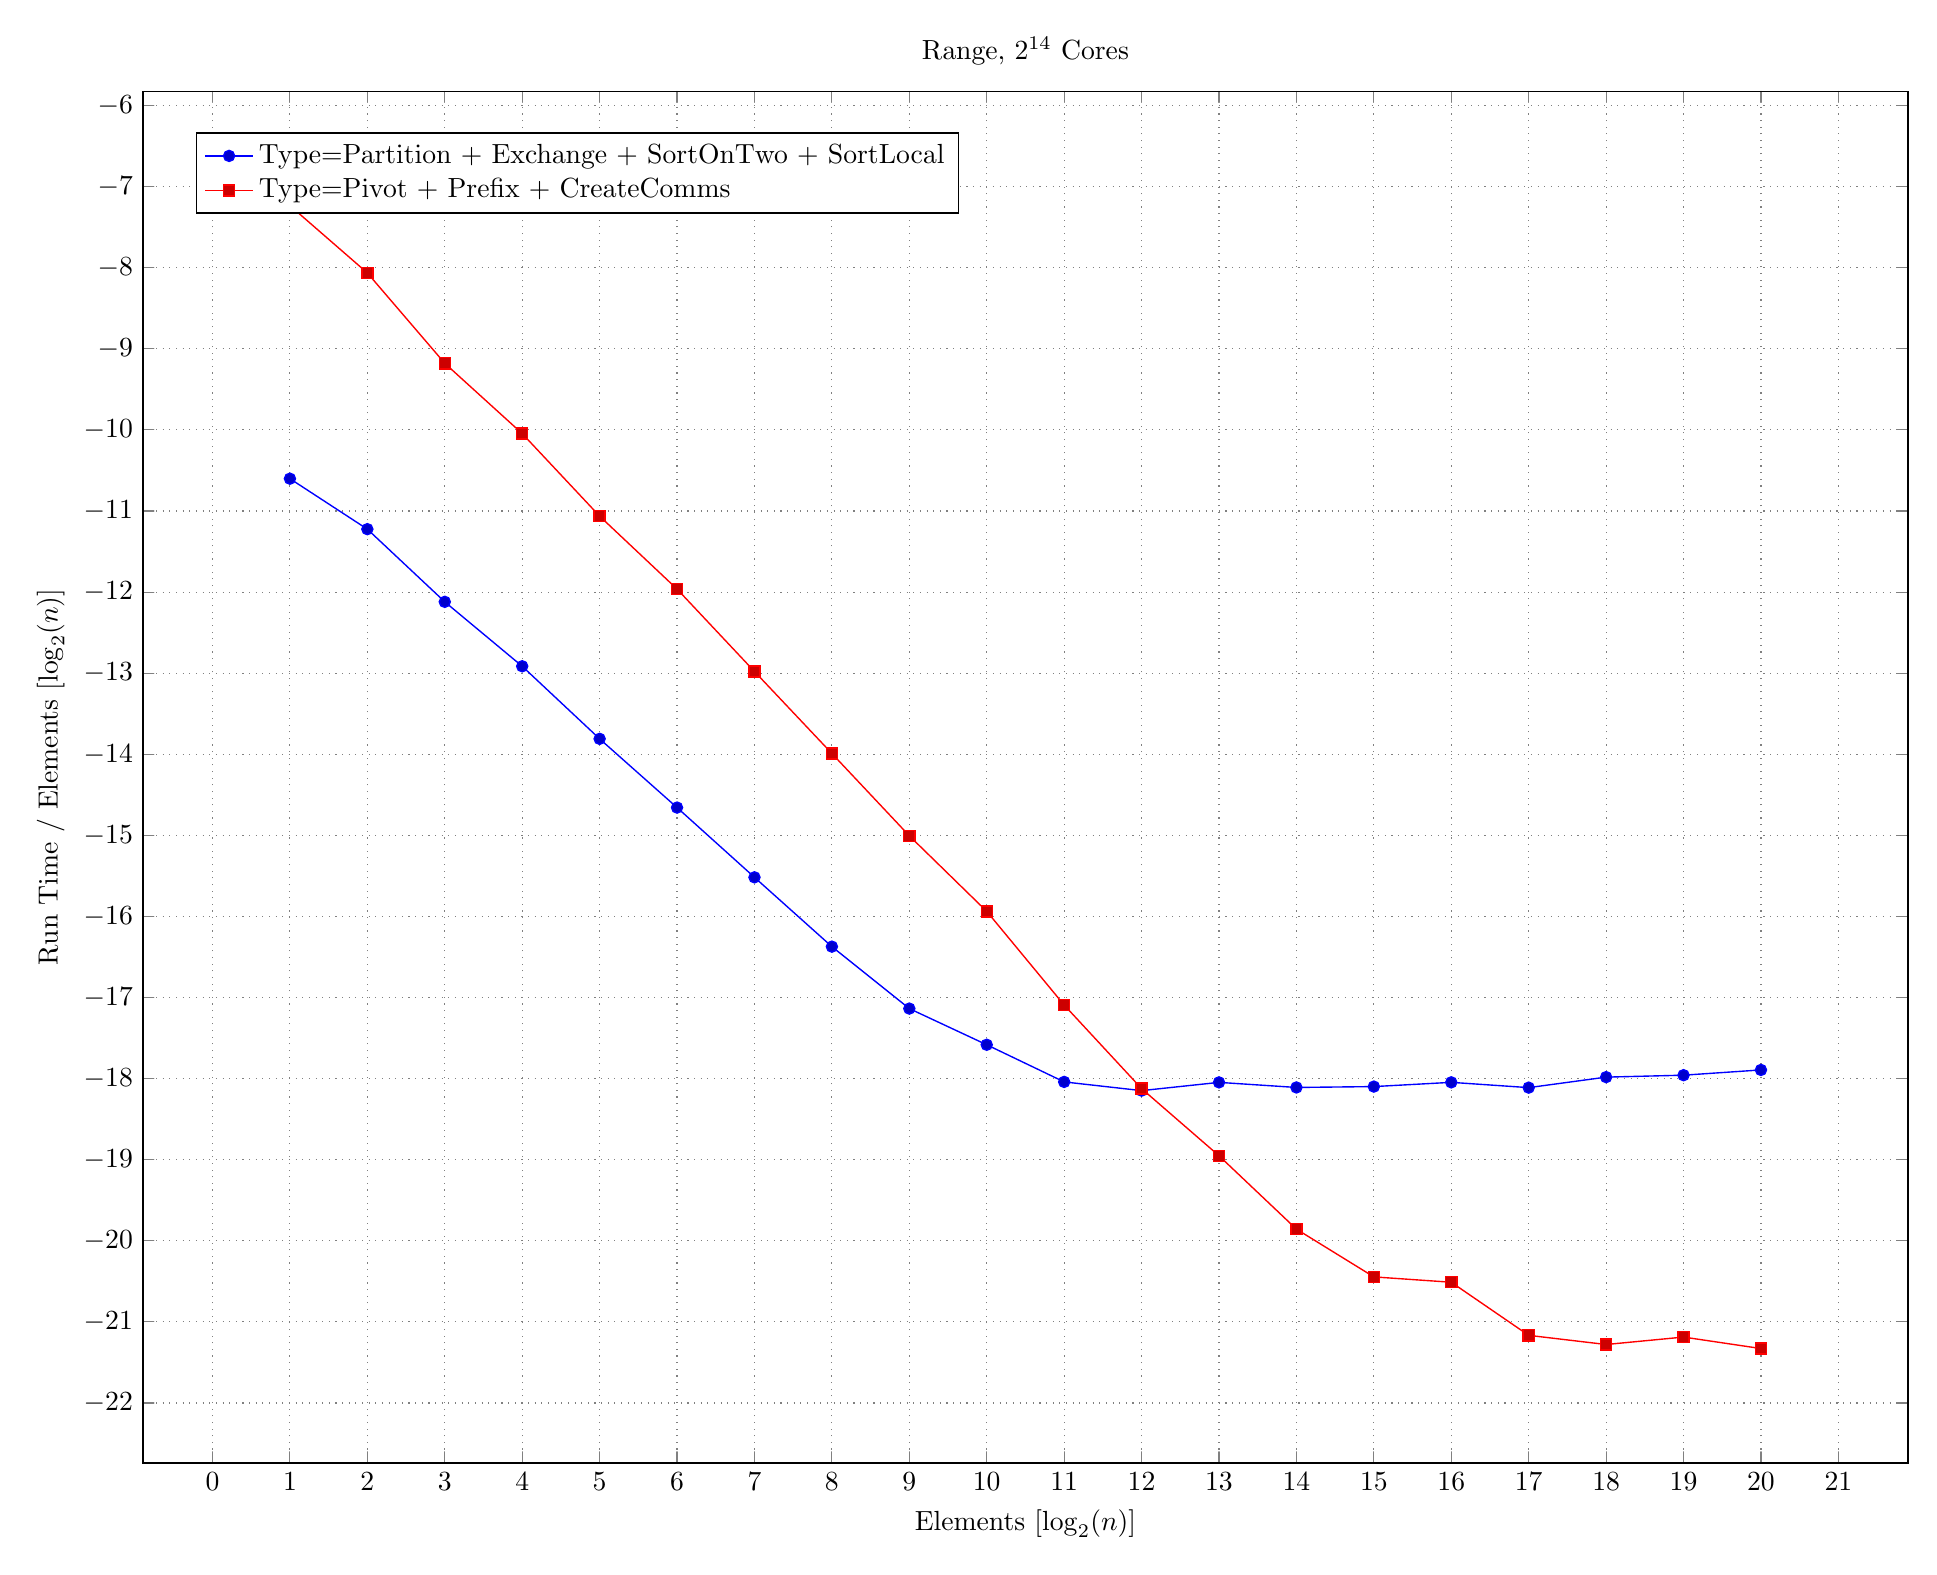
\begin{tikzpicture}
  \begin{axis}[
    title={Range, $2^{14}$ Cores},
    xlabel={Elements [$\log_2(n)$]},
    ylabel={Run Time / Elements [$\log_2(n)$]},
    ]   
	%% MULTIPLOT(Type) SELECT size, collective, LOG(2,elements) AS x, LOG(2,Time/elements) as y, MULTIPLOT FROM (    
	%% SELECT elements, size, MEDIAN(pivot + calculate + create_comms) as Time, 'Pivot + Prefix + CreateComms' as Type, collective, blocking, mpi_split
	%% FROM ResultsQS
	%% GROUP BY collective, size, elements, blocking, mpi_split
	%% UNION ALL
	%% SELECT elements, size, MEDIAN(partition + exchange + sort_two + sort_local) as Time, 'Partition + Exchange + SortOnTwo + SortLocal' as Type, collective, blocking, mpi_split
	%% FROM ResultsQS
	%% GROUP BY collective, size, elements, blocking, mpi_split
	%% ) a
	%% WHERE collective="range" AND size=16384 AND blocking=0 AND mpi_split=0 
	%% GROUP BY MULTIPLOT, x  ORDER BY MULTIPLOT, x
 \addplot coordinates { (1.0,-10.6017) (2.0,-11.2242) (3.0,-12.1203) (4.0,-12.9149) (5.0,-13.8097) (6.0,-14.6573) (7.0,-15.5174) (8.0,-16.3722) (9.0,-17.1361) (10.0,-17.5823) (11.0,-18.0403) (12.0,-18.1477) (13.0,-18.0461) (14.0,-18.1087) (15.0,-18.0979) (16.0,-18.0457) (17.0,-18.1108) (18.0,-17.9813) (19.0,-17.9574) (20.0,-17.8926) };
 \addlegendentry{Type=Partition + Exchange + SortOnTwo + SortLocal};
 \addplot coordinates { (1.0,-7.23434) (2.0,-8.06456) (3.0,-9.17895) (4.0,-10.0456) (5.0,-11.0637) (6.0,-11.963) (7.0,-12.9791) (8.0,-13.9905) (9.0,-15.0055) (10.0,-15.9372) (11.0,-17.0924) (12.0,-18.1229) (13.0,-18.9512) (14.0,-19.8558) (15.0,-20.4446) (16.0,-20.5107) (17.0,-21.1654) (18.0,-21.2785) (19.0,-21.1867) (20.0,-21.3283) };
 \addlegendentry{Type=Pivot + Prefix + CreateComms};


  \end{axis}
\end{tikzpicture}
\newpage

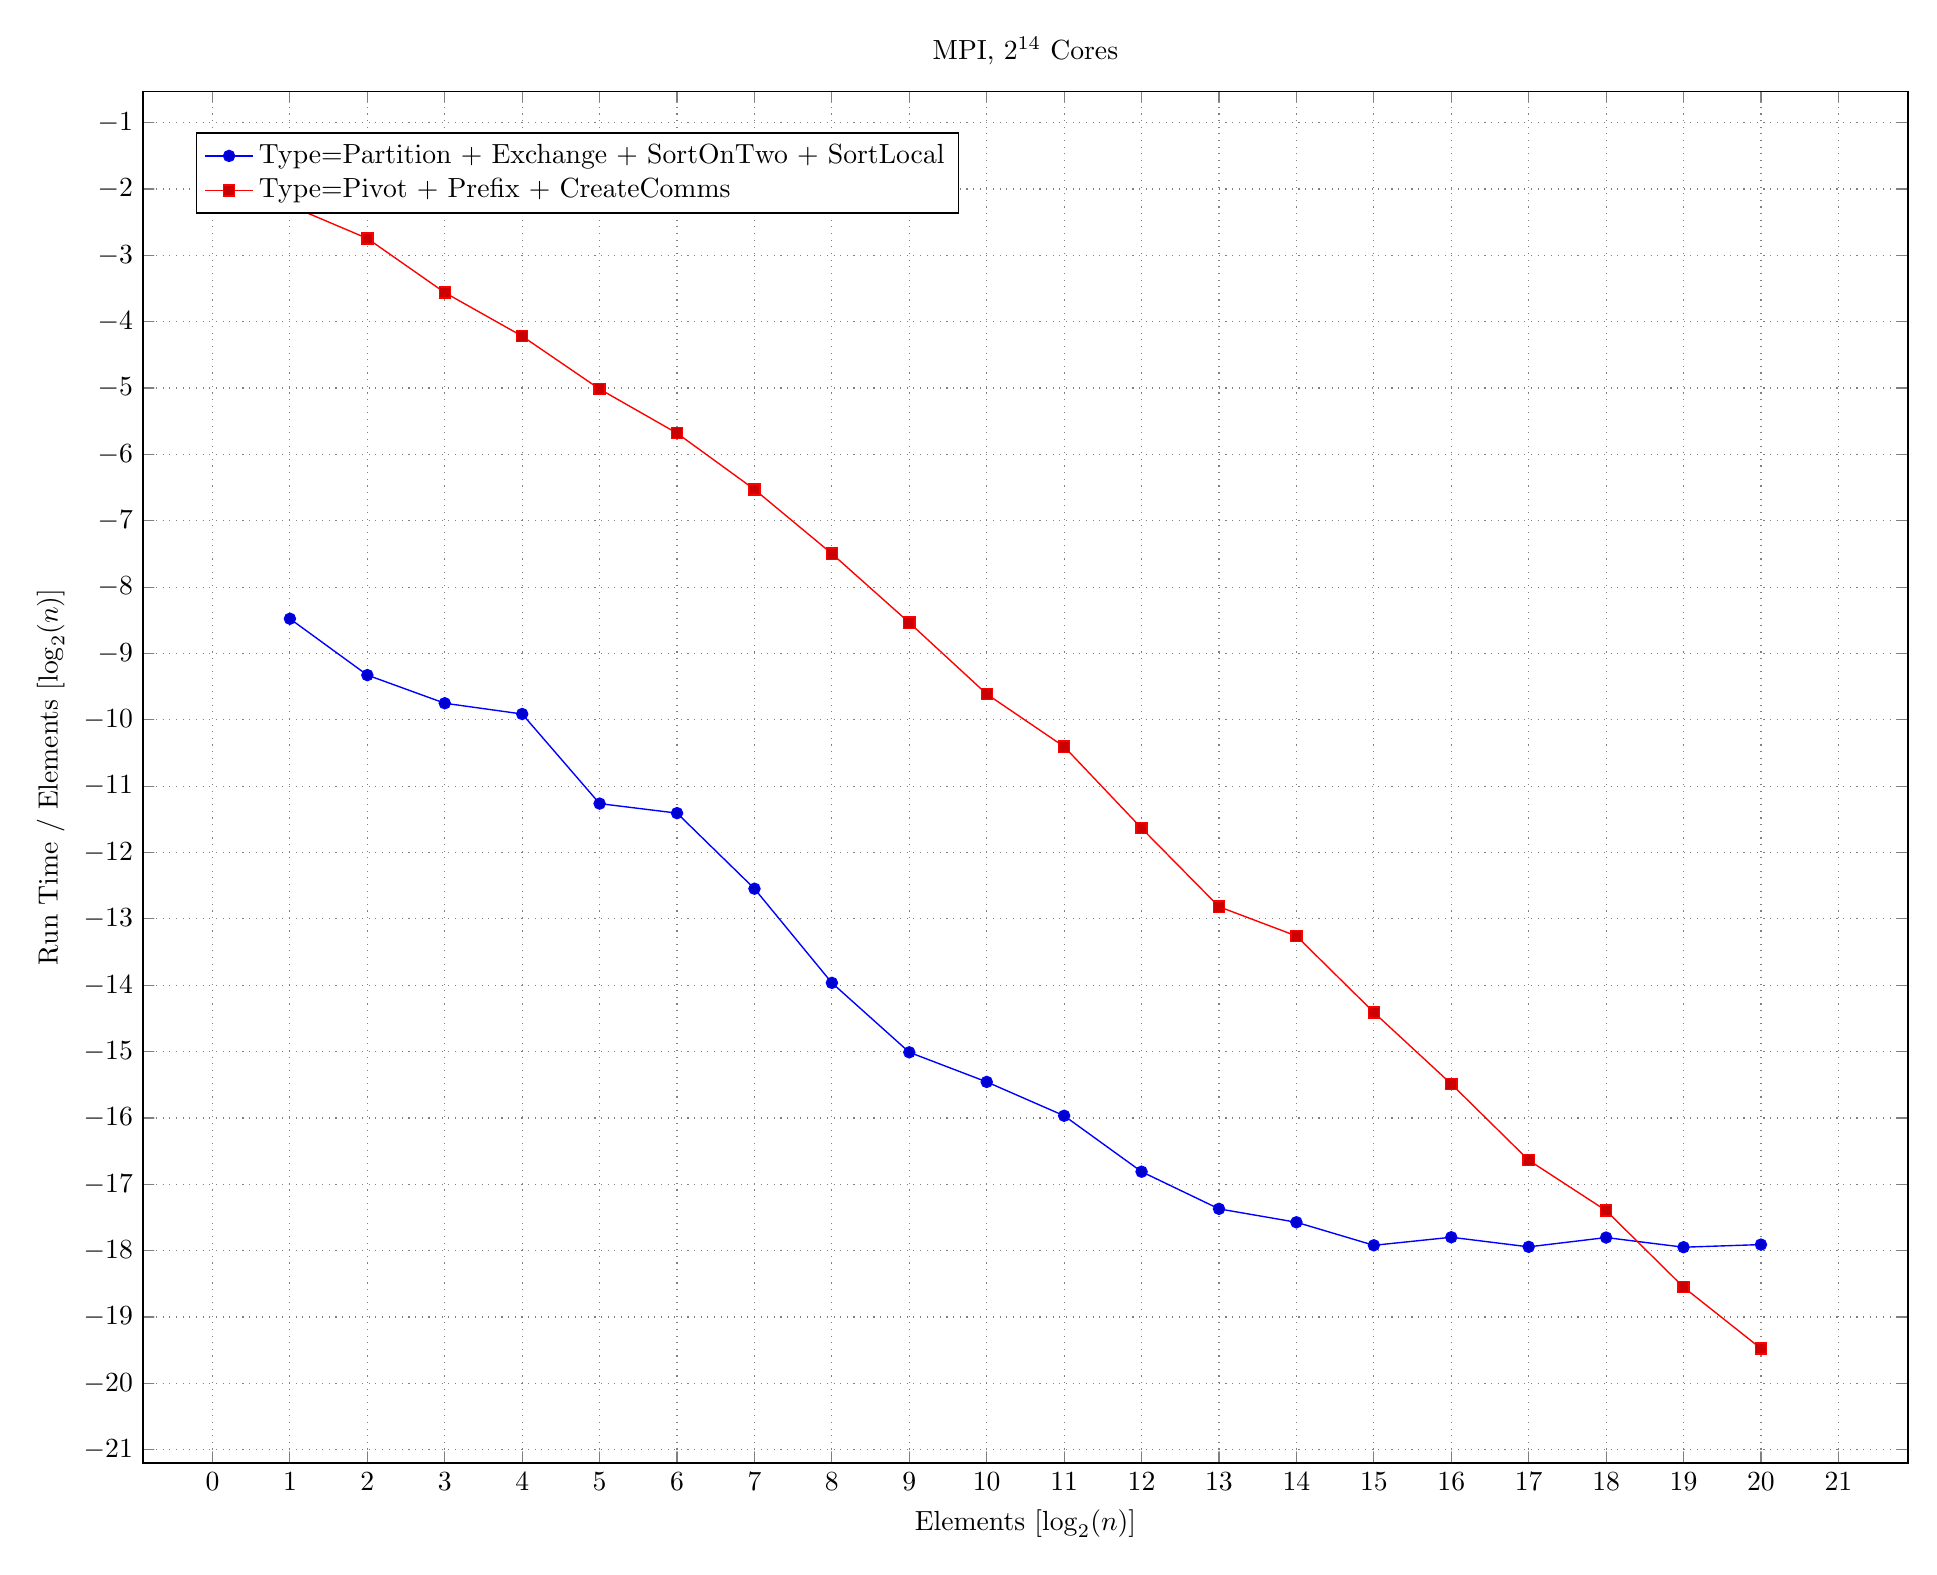
\begin{tikzpicture}
  \begin{axis}[
    title={MPI, $2^{14}$ Cores},
    xlabel={Elements [$\log_2(n)$]},
    ylabel={Run Time / Elements [$\log_2(n)$]},
    ]   
	%% MULTIPLOT(Type) SELECT size, collective, LOG(2,elements) AS x, LOG(2,Time/elements) as y, MULTIPLOT FROM (    
	%% SELECT elements, size, MEDIAN(pivot + calculate + create_comms) as Time, 'Pivot + Prefix + CreateComms' as Type, collective, blocking, mpi_split
	%% FROM ResultsQS
	%% GROUP BY collective, size, elements, blocking, mpi_split
	%% UNION ALL
	%% SELECT elements, size, MEDIAN(partition + exchange + sort_two + sort_local) as Time, 'Partition + Exchange + SortOnTwo + SortLocal' as Type, collective, blocking, mpi_split
	%% FROM ResultsQS
	%% GROUP BY collective, size, elements, blocking, mpi_split
	%% ) a
	%% WHERE collective="mpi" AND size=16384 AND blocking=1 AND mpi_split=1
	%% GROUP BY MULTIPLOT, x  ORDER BY MULTIPLOT, x
 \addplot coordinates { (1.0,-8.4768) (2.0,-9.3261) (3.0,-9.75002) (4.0,-9.9123) (5.0,-11.2625) (6.0,-11.4059) (7.0,-12.5451) (8.0,-13.9641) (9.0,-15.0104) (10.0,-15.4566) (11.0,-15.9666) (12.0,-16.8097) (13.0,-17.3698) (14.0,-17.5716) (15.0,-17.9188) (16.0,-17.7975) (17.0,-17.9421) (18.0,-17.8019) (19.0,-17.9475) (20.0,-17.9079) };
 \addlegendentry{Type=Partition + Exchange + SortOnTwo + SortLocal};
 \addplot coordinates { (1.0,-2.25067) (2.0,-2.7457) (3.0,-3.56153) (4.0,-4.21824) (5.0,-5.01562) (6.0,-5.68093) (7.0,-6.52787) (8.0,-7.49636) (9.0,-8.53617) (10.0,-9.61186) (11.0,-10.4044) (12.0,-11.6337) (13.0,-12.8163) (14.0,-13.2573) (15.0,-14.4087) (16.0,-15.4879) (17.0,-16.6364) (18.0,-17.396) (19.0,-18.5499) (20.0,-19.4747) };
 \addlegendentry{Type=Pivot + Prefix + CreateComms};


  \end{axis}
\end{tikzpicture}
\newpage

\begin{tikzpicture}
  \begin{axis}[
    title={MPI, $2^{14}$ Cores},
    xlabel={Elements [$\log_2(n)$]},
    ylabel={Run Time},
    ]   
	%% MULTIPLOT(Type) SELECT size, collective, LOG(2,elements) AS x, Time as y, MULTIPLOT FROM (  
	%% SELECT elements, size, MEDIAN(create_comms) as Time, 'Create Comms' as Type, collective, blocking, mpi_split
	%% FROM ResultsQS
	%% GROUP BY collective, size, elements, blocking, mpi_split
	%% UNION ALL
	%% SELECT elements, size, MEDIAN(sum - create_comms) as Time, 'Sum - Create Comms' as Type, collective, blocking, mpi_split
	%% FROM ResultsQS
	%% GROUP BY collective, size, elements, blocking, mpi_split
	%% ) a
	%% WHERE collective="mpi" AND size=16384 AND blocking=1 AND mpi_split=1
	%% GROUP BY MULTIPLOT, x  ORDER BY MULTIPLOT, x
 \addplot coordinates { (1.0,0.386326) (2.0,0.544804) (3.0,0.620089) (4.0,0.797368) (5.0,0.917367) (6.0,1.17111) (7.0,1.31332) (8.0,1.33105) (9.0,1.30852) (10.0,1.24128) (11.0,1.44304) (12.0,1.22469) (13.0,1.06228) (14.0,1.57684) (15.0,1.43692) (16.0,1.34795) (17.0,1.205) (18.0,1.43176) (19.0,1.2294) (20.0,1.16678) };
 \addlegendentry{Type=Create Comms};
 \addplot coordinates { (1.0,0.038399) (2.0,0.05811) (3.0,0.066646) (4.0,0.078413) (5.0,0.084913) (6.0,0.1111) (7.0,0.09503) (8.0,0.08482) (9.0,0.08597) (10.0,0.09316) (11.0,0.14423) (12.0,0.10281) (13.0,0.12333) (14.0,0.16932) (15.0,0.20783) (16.0,0.36987) (17.0,0.60603) (18.0,1.24446) (19.0,2.2384) (20.0,4.5701) };
 \addlegendentry{Type=Sum - Create Comms};


  \end{axis}
\end{tikzpicture}
\newpage

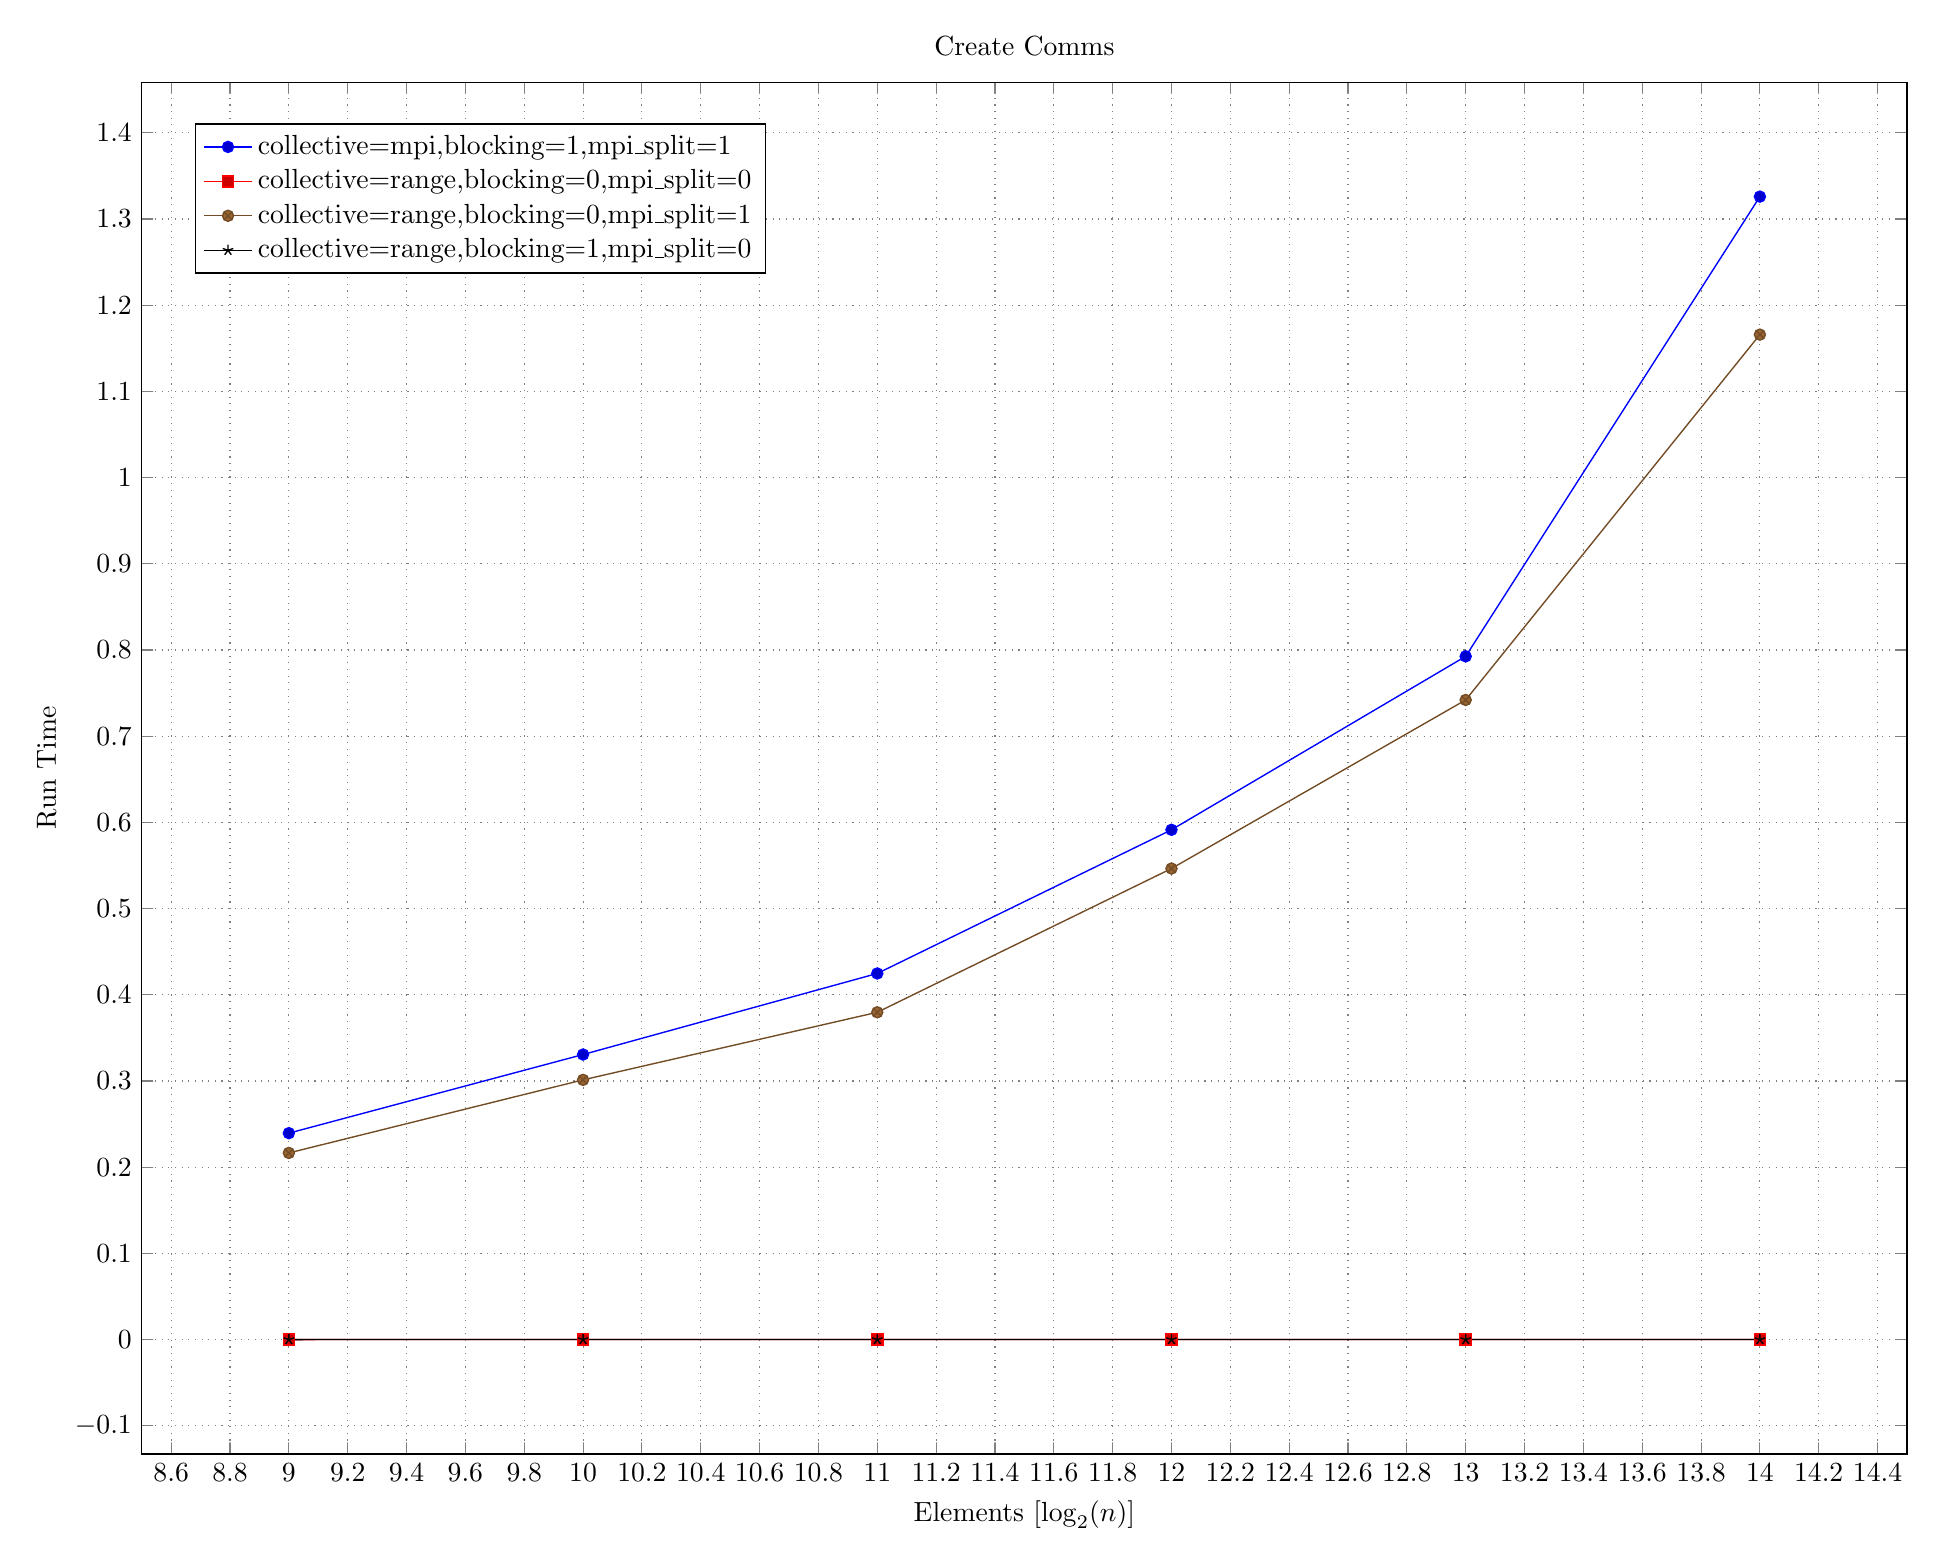
\begin{tikzpicture}
  \begin{axis}[
    title={Create Comms},
    xlabel={Elements [$\log_2(n)$]},
    ylabel={Run Time},
    ]   
	%% MULTIPLOT(collective, blocking, mpi_split) SELECT LOG(2,size) AS x, MEDIAN(create_comms) as y, MULTIPLOT
	%% FROM ResultsQS
	%% WHERE elements>POWER(2,5) AND elements<POWER(2,20)
	%% GROUP BY MULTIPLOT, x  ORDER BY MULTIPLOT, x
 \addplot coordinates { (9.0,0.239471) (10.0,0.330703) (11.0,0.424748) (12.0,0.59142) (13.0,0.792665) (14.0,1.32603) };
 \addlegendentry{collective=mpi,blocking=1,mpi\_split=1};
 \addplot coordinates { (9.0,1.98e-05) (10.0,2.238e-05) (11.0,2.39119e-05) (12.0,2.66275e-05) (13.0,2.96228e-05) (14.0,3.12568e-05) };
 \addlegendentry{collective=range,blocking=0,mpi\_split=0};
 \addplot coordinates { (9.0,0.216522) (10.0,0.301309) (11.0,0.37971) (12.0,0.546482) (13.0,0.74207) (14.0,1.165935) };
 \addlegendentry{collective=range,blocking=0,mpi\_split=1};
 \addplot coordinates { (9.0,1.99516e-05) (10.0,2.27194e-05) (11.0,2.42259e-05) (12.0,2.63944e-05) (13.0,2.92278e-05) (14.0,3.12559e-05) };
 \addlegendentry{collective=range,blocking=1,mpi\_split=0};


  \end{axis}
\end{tikzpicture}
\newpage

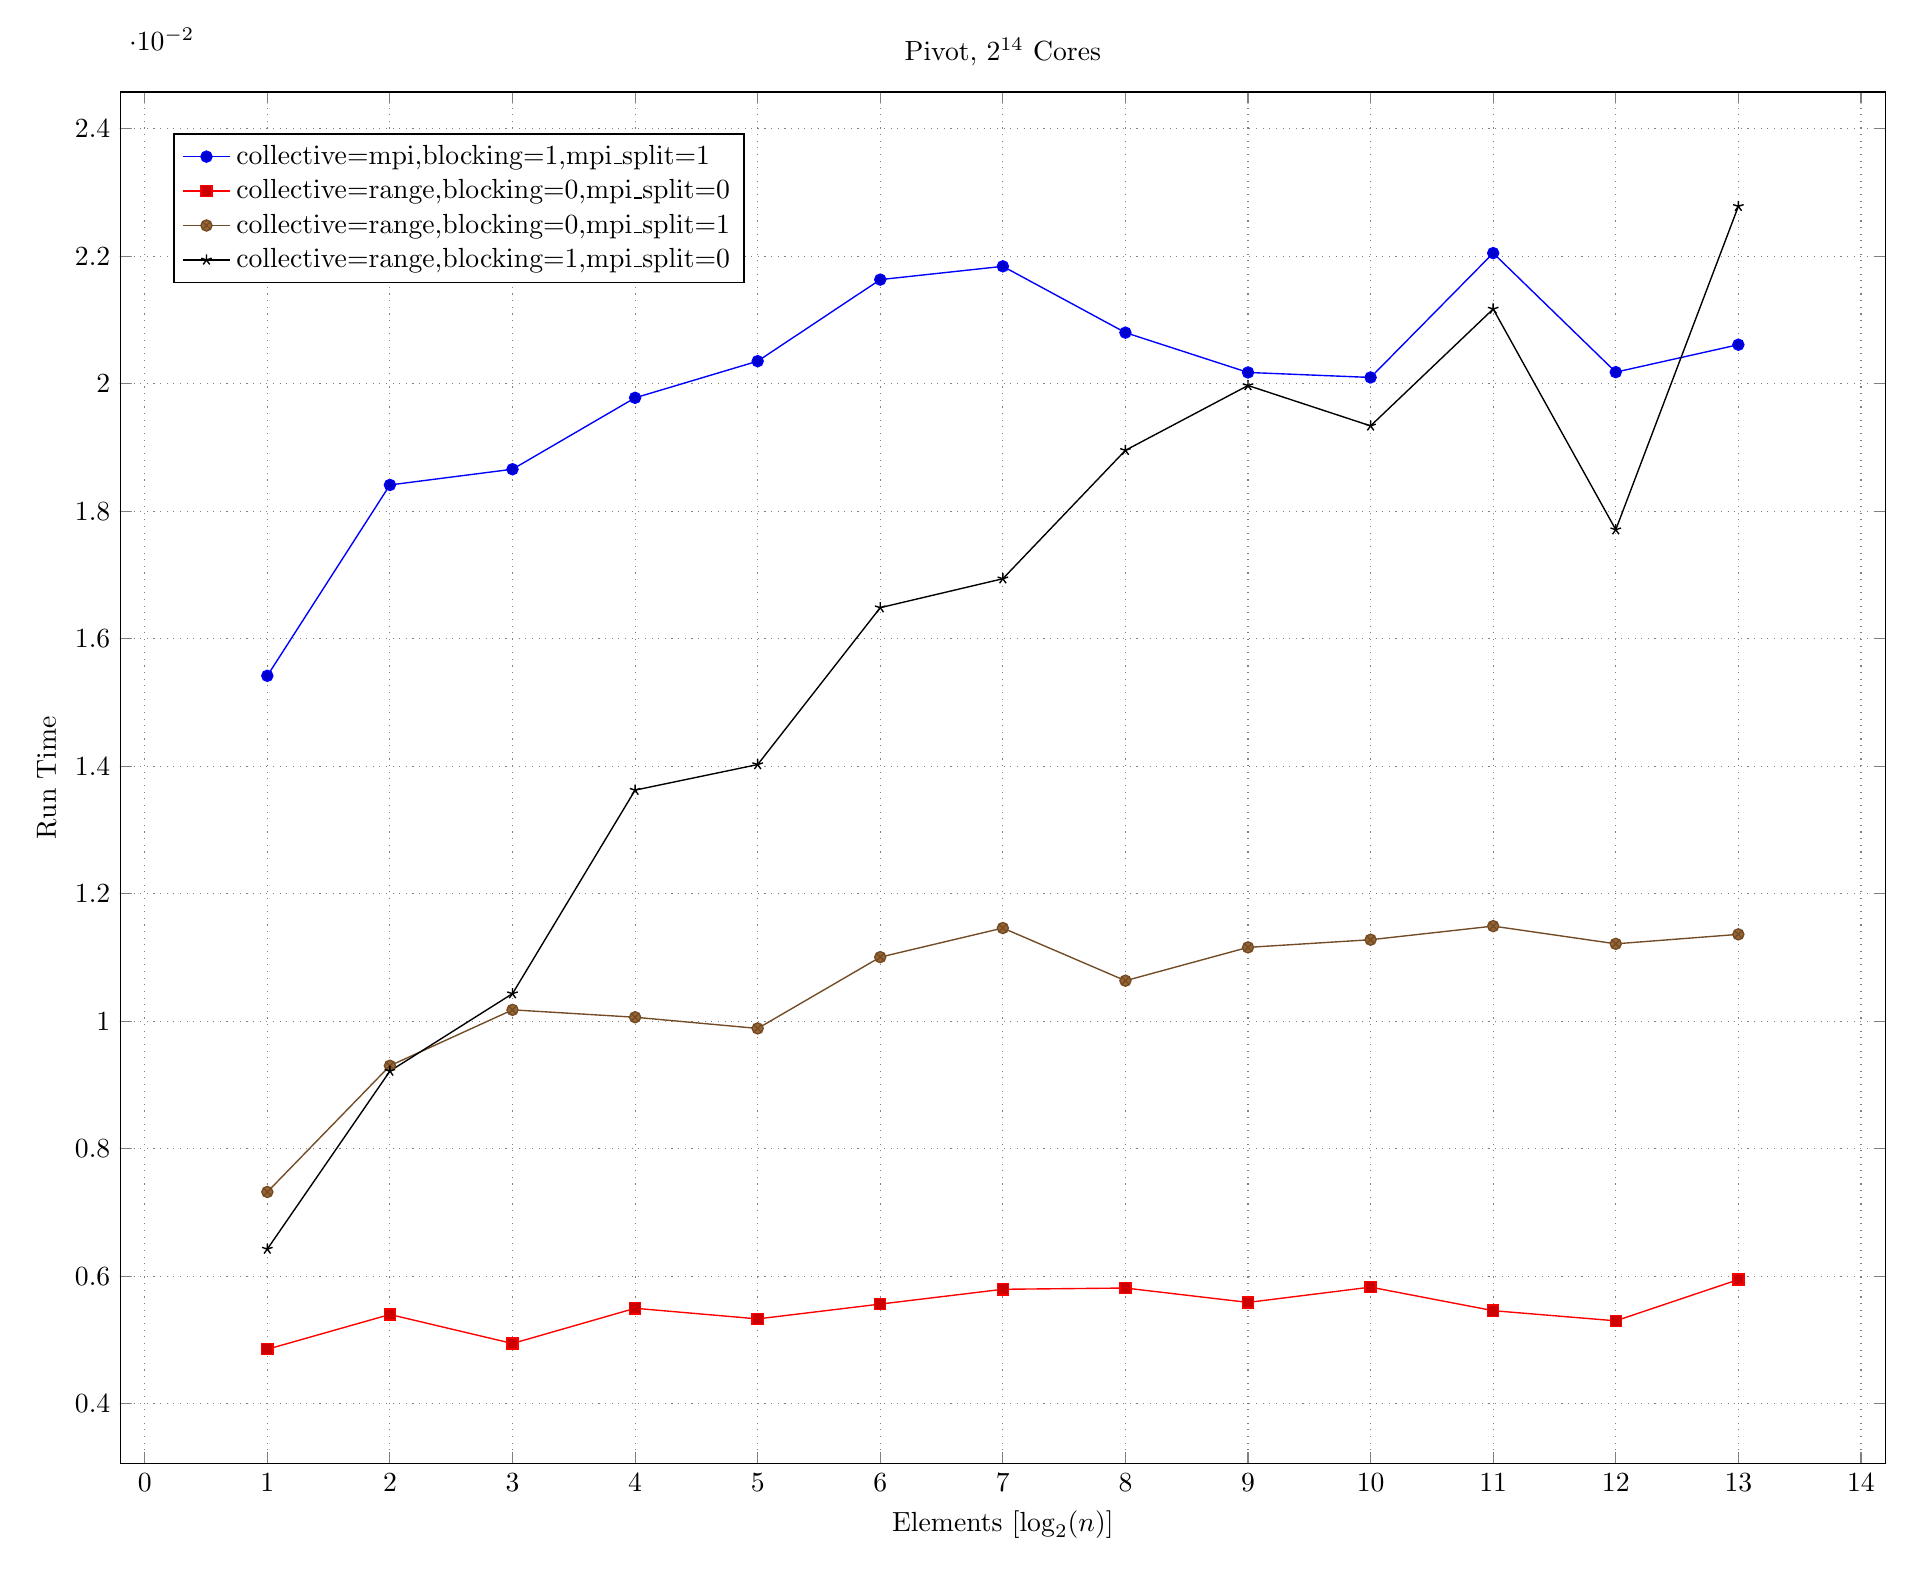
\begin{tikzpicture}
  \begin{axis}[
    title={Pivot, $2^{14}$ Cores},
    xlabel={Elements [$\log_2(n)$]},
    ylabel={Run Time},
    ]   
	%% MULTIPLOT(collective, blocking, mpi_split) SELECT LOG(2,elements) AS x, MEDIAN(pivot) as y, MULTIPLOT
	%% FROM ResultsQS
	%% WHERE size=16384 AND x<14
	%% GROUP BY MULTIPLOT, x  ORDER BY MULTIPLOT, x
 \addplot coordinates { (1.0,0.0154193) (2.0,0.0184123) (3.0,0.0186587) (4.0,0.0197787) (5.0,0.0203535) (6.0,0.0216326) (7.0,0.0218407) (8.0,0.020801) (9.0,0.0201766) (10.0,0.0200981) (11.0,0.0220483) (12.0,0.0201813) (13.0,0.0206116) };
 \addlegendentry{collective=mpi,blocking=1,mpi\_split=1};
 \addplot coordinates { (1.0,0.00485747) (2.0,0.0054029) (3.0,0.00494767) (4.0,0.00550004) (5.0,0.00533361) (6.0,0.00556592) (7.0,0.00579797) (8.0,0.00581752) (9.0,0.00559205) (10.0,0.00583175) (11.0,0.00546249) (12.0,0.00530344) (13.0,0.00594981) };
 \addlegendentry{collective=range,blocking=0,mpi\_split=0};
 \addplot coordinates { (1.0,0.00732419) (2.0,0.00930388) (3.0,0.0101804) (4.0,0.0100644) (5.0,0.00988873) (6.0,0.0110072) (7.0,0.0114632) (8.0,0.0106374) (9.0,0.0111602) (10.0,0.0112803) (11.0,0.0114935) (12.0,0.0112158) (13.0,0.0113643) };
 \addlegendentry{collective=range,blocking=0,mpi\_split=1};
 \addplot coordinates { (1.0,0.00642867) (2.0,0.00922015) (3.0,0.0104344) (4.0,0.0136261) (5.0,0.0140272) (6.0,0.0164875) (7.0,0.0169415) (8.0,0.0189553) (9.0,0.0199716) (10.0,0.0193387) (11.0,0.0211715) (12.0,0.0177101) (13.0,0.0227819) };
 \addlegendentry{collective=range,blocking=1,mpi\_split=0};


  \end{axis}
\end{tikzpicture}
\newpage

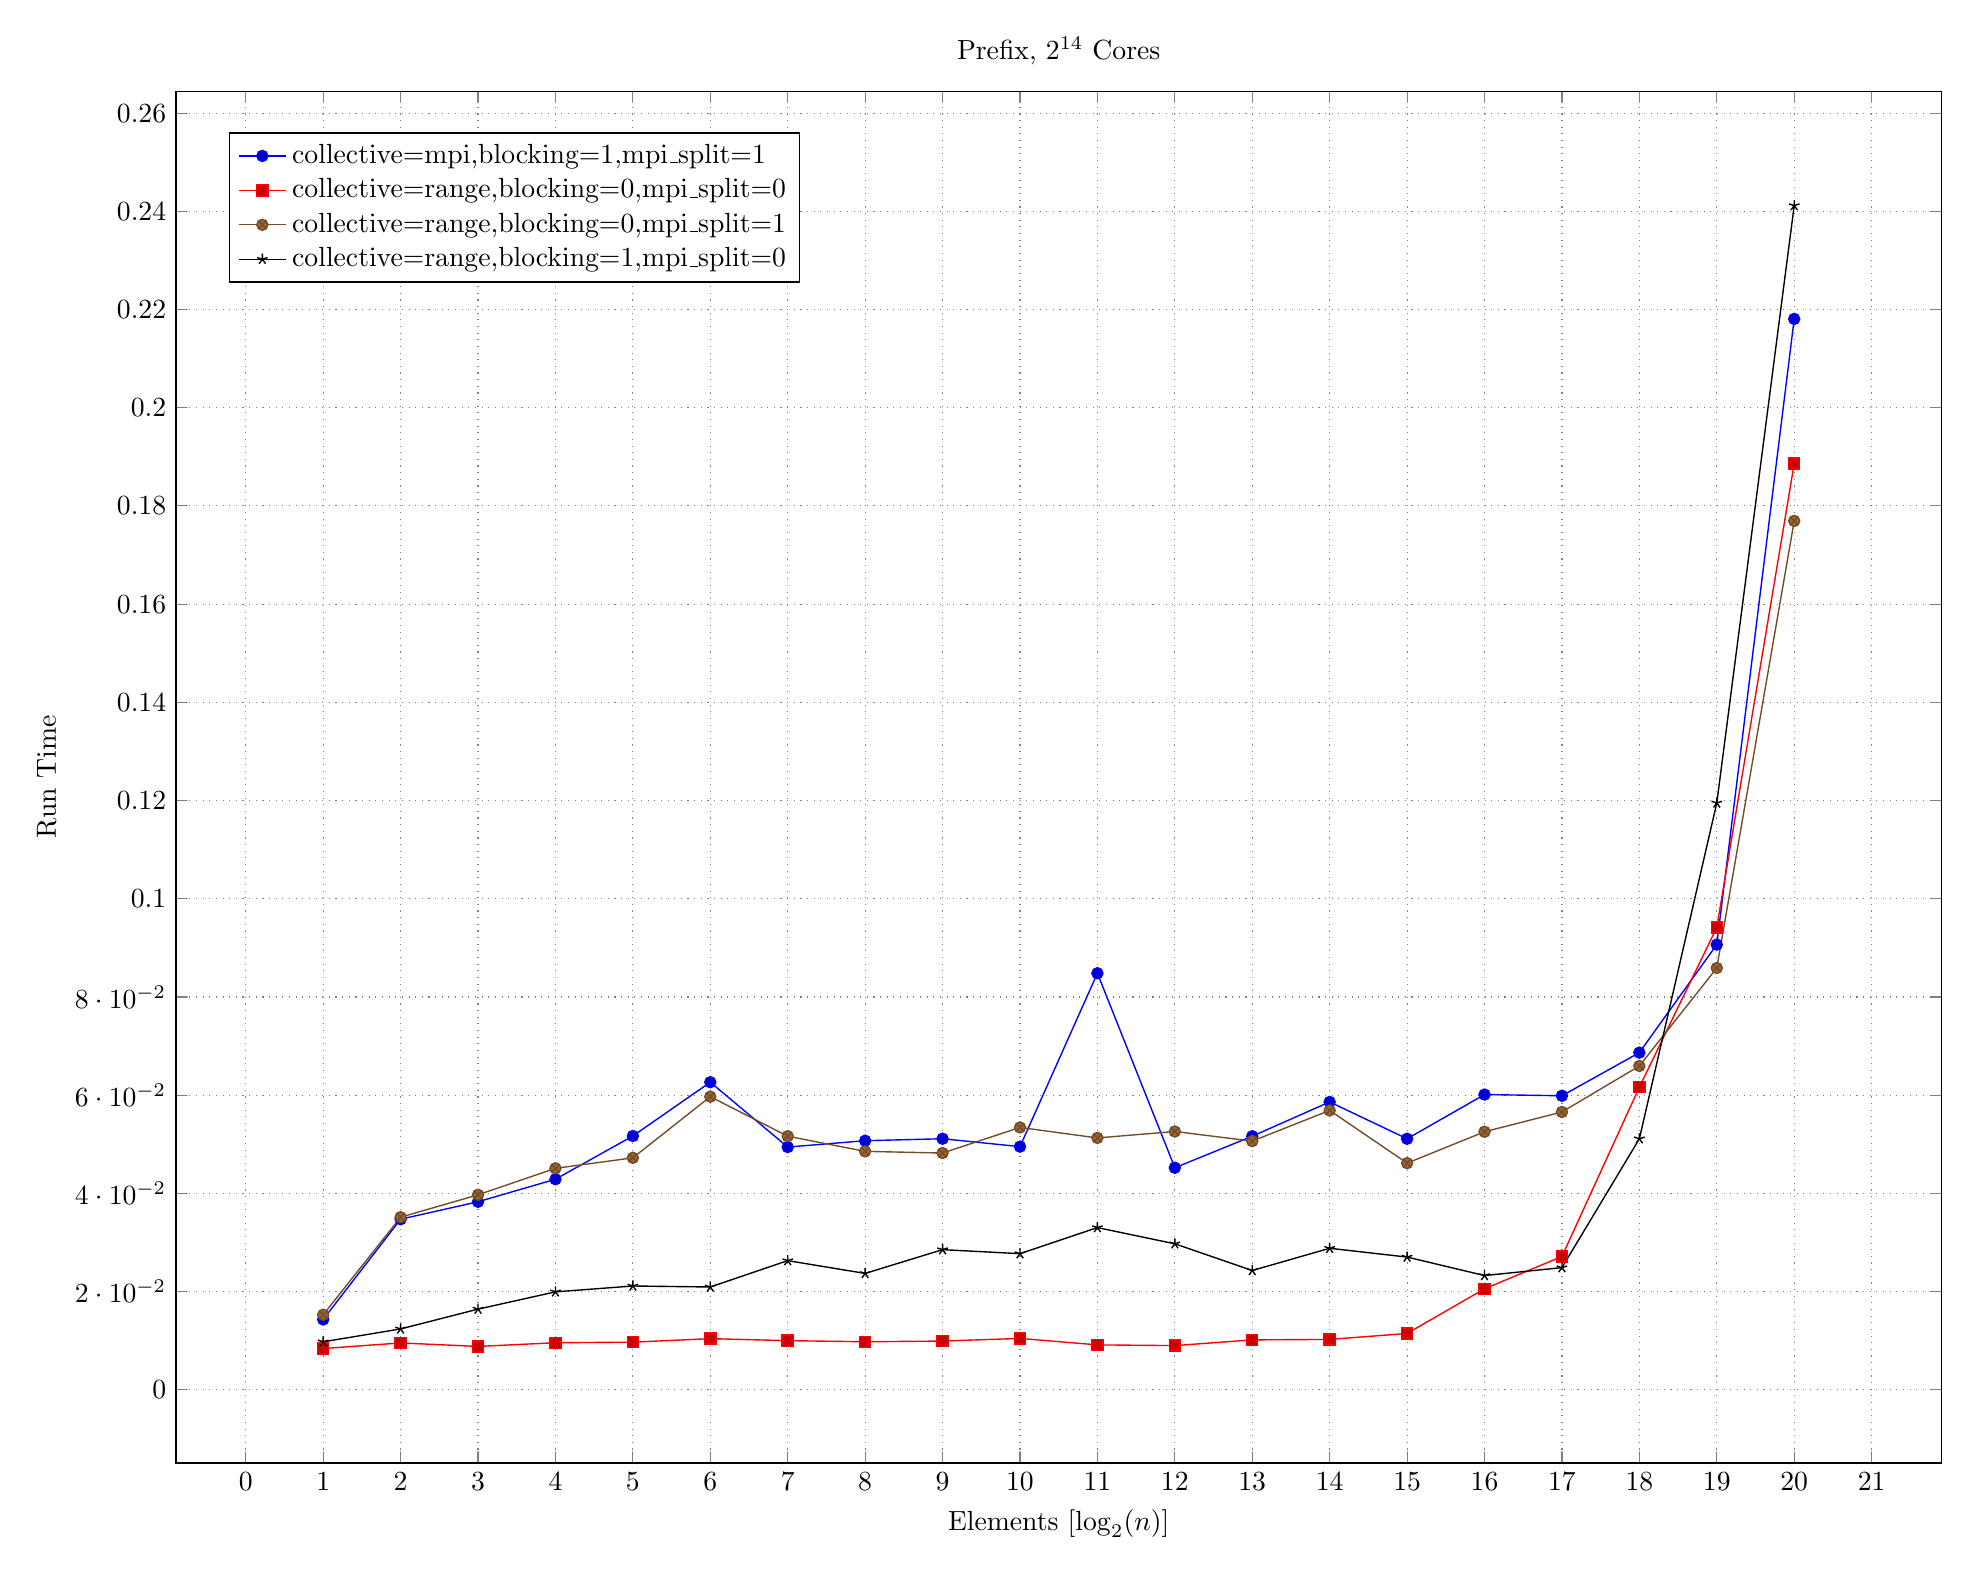
\begin{tikzpicture}
  \begin{axis}[
    title={Prefix, $2^{14}$ Cores},
    xlabel={Elements [$\log_2(n)$]},
    ylabel={Run Time},
    ]   
	%% MULTIPLOT(collective, blocking, mpi_split) SELECT LOG(2,elements) AS x, MEDIAN(calculate) as y, MULTIPLOT
	%% FROM ResultsQS
	%% WHERE size=16384
	%% GROUP BY MULTIPLOT, x  ORDER BY MULTIPLOT, x
 \addplot coordinates { (1.0,0.014338) (2.0,0.0347583) (3.0,0.0383056) (4.0,0.0428972) (5.0,0.0517009) (6.0,0.0626571) (7.0,0.0494455) (8.0,0.0507386) (9.0,0.0511406) (10.0,0.0495332) (11.0,0.0848411) (12.0,0.0452296) (13.0,0.0516538) (14.0,0.0586342) (15.0,0.0511333) (16.0,0.0601391) (17.0,0.0598941) (18.0,0.0686769) (19.0,0.09068) (20.0,0.218083) };
 \addlegendentry{collective=mpi,blocking=1,mpi\_split=1};
 \addplot coordinates { (1.0,0.00841656) (2.0,0.00956046) (3.0,0.0088472) (4.0,0.00960087) (5.0,0.00971691) (6.0,0.0104338) (7.0,0.0100232) (8.0,0.0098007) (9.0,0.00994269) (10.0,0.0104784) (11.0,0.00916407) (12.0,0.00901633) (13.0,0.010181) (14.0,0.0102762) (15.0,0.0114923) (16.0,0.0205767) (17.0,0.027164) (18.0,0.0616457) (19.0,0.0941636) (20.0,0.188622) };
 \addlegendentry{collective=range,blocking=0,mpi\_split=0};
 \addplot coordinates { (1.0,0.0152883) (2.0,0.0351637) (3.0,0.0397236) (4.0,0.0451129) (5.0,0.0472523) (6.0,0.059711) (7.0,0.051654) (8.0,0.0485728) (9.0,0.0482295) (10.0,0.0534417) (11.0,0.0513066) (12.0,0.0526171) (13.0,0.050658) (14.0,0.0569082) (15.0,0.0461738) (16.0,0.052563) (17.0,0.056587) (18.0,0.0659592) (19.0,0.0859115) (20.0,0.176949) };
 \addlegendentry{collective=range,blocking=0,mpi\_split=1};
 \addplot coordinates { (1.0,0.00978485) (2.0,0.0124099) (3.0,0.0164426) (4.0,0.0199608) (5.0,0.021154) (6.0,0.0209524) (7.0,0.0263177) (8.0,0.0237164) (9.0,0.028555) (10.0,0.0277372) (11.0,0.0330495) (12.0,0.029746) (13.0,0.0243084) (14.0,0.0288354) (15.0,0.0270457) (16.0,0.0232819) (17.0,0.0248953) (18.0,0.0511311) (19.0,0.119514) (20.0,0.241158) };
 \addlegendentry{collective=range,blocking=1,mpi\_split=0};


  \end{axis}
\end{tikzpicture}
\newpage

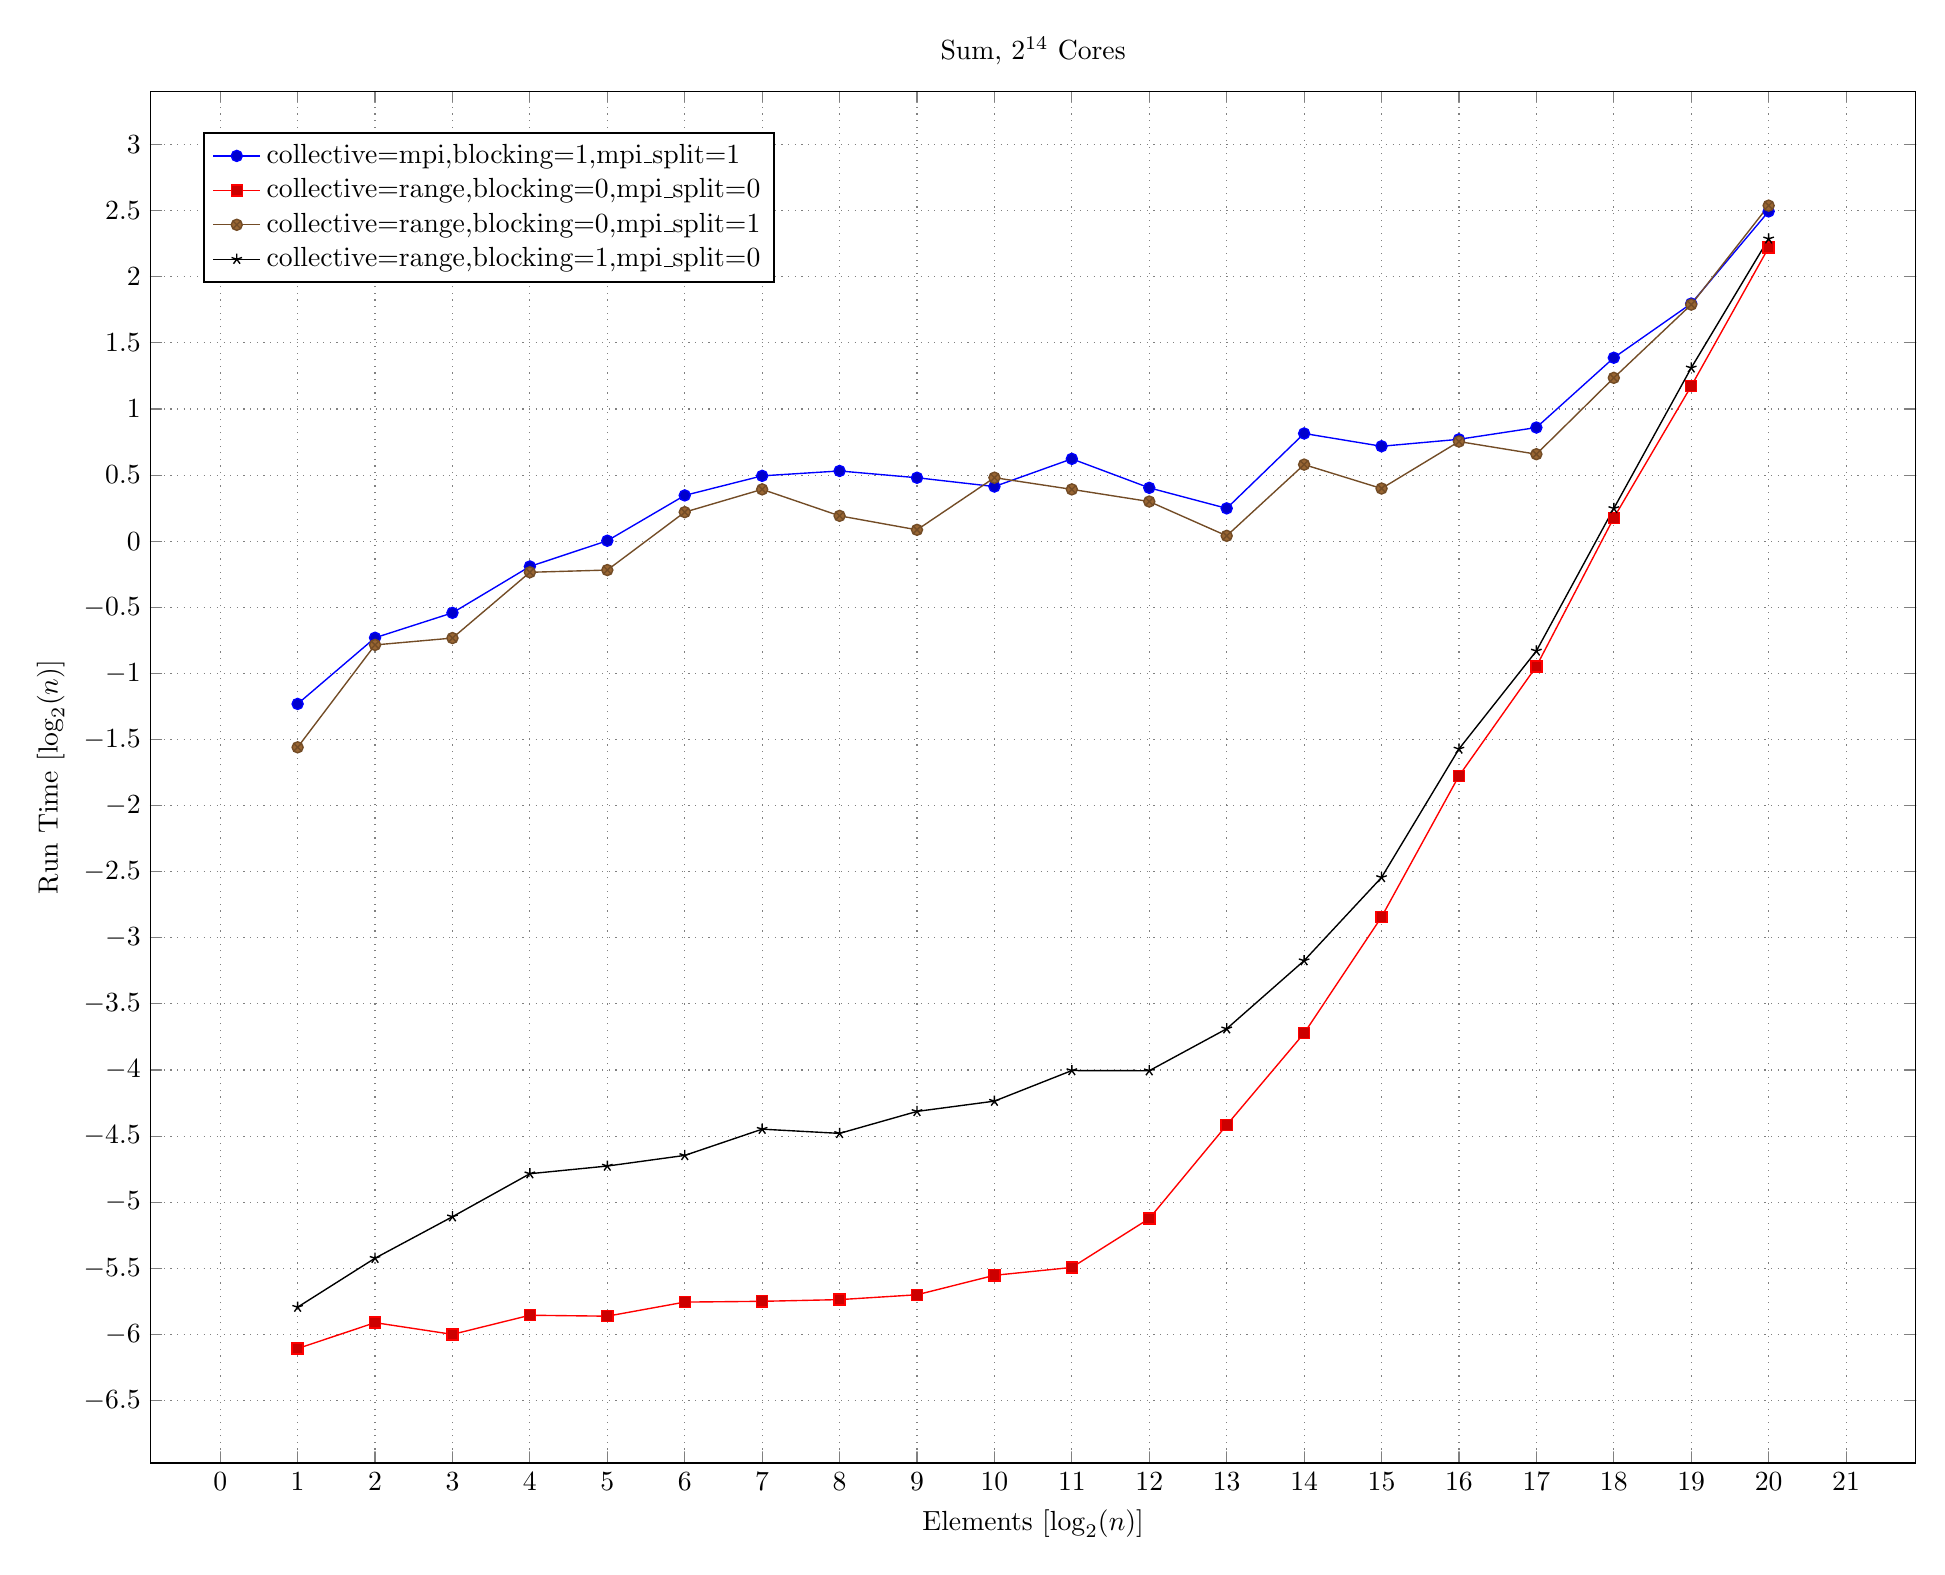
\begin{tikzpicture}
  \begin{axis}[
    title={Sum, $2^{14}$ Cores},
    xlabel={Elements [$\log_2(n)$]},
    ylabel={Run Time [$\log_2(n)$]},
    ]   
	%% MULTIPLOT(collective, blocking, mpi_split) SELECT LOG(2,elements) AS x, LOG(2,MEDIAN(sum)) as y, MULTIPLOT
	%% FROM ResultsQS
	%% WHERE size=16384
	%% GROUP BY MULTIPLOT, x  ORDER BY MULTIPLOT, x
 \addplot coordinates { (1.0,-1.23106) (2.0,-0.730703) (3.0,-0.542175) (4.0,-0.191358) (5.0,0.0032856) (6.0,0.346089) (7.0,0.494078) (8.0,0.53105) (9.0,0.479738) (10.0,0.413031) (11.0,0.622631) (12.0,0.403322) (13.0,0.248134) (14.0,0.814567) (15.0,0.717868) (16.0,0.770491) (17.0,0.859516) (18.0,1.38739) (19.0,1.79723) (20.0,2.49438) };
 \addlegendentry{collective=mpi,blocking=1,mpi\_split=1};
 \addplot coordinates { (1.0,-6.10721) (2.0,-5.9113) (3.0,-6.00003) (4.0,-5.85525) (5.0,-5.86239) (6.0,-5.75577) (7.0,-5.74991) (8.0,-5.73707) (9.0,-5.70031) (10.0,-5.55325) (11.0,-5.49366) (12.0,-5.12376) (13.0,-4.41677) (14.0,-3.7221) (15.0,-2.84255) (16.0,-1.77549) (17.0,-0.946875) (18.0,0.176246) (19.0,1.17313) (20.0,2.22133) };
 \addlegendentry{collective=range,blocking=0,mpi\_split=0};
 \addplot coordinates { (1.0,-1.55938) (2.0,-0.78493) (3.0,-0.733006) (4.0,-0.235472) (5.0,-0.218508) (6.0,0.219574) (7.0,0.391867) (8.0,0.191525) (9.0,0.0857238) (10.0,0.480317) (11.0,0.391702) (12.0,0.299737) (13.0,0.0402612) (14.0,0.579161) (15.0,0.398285) (16.0,0.753416) (17.0,0.657978) (18.0,1.23543) (19.0,1.78925) (20.0,2.5382) };
 \addlegendentry{collective=range,blocking=0,mpi\_split=1};
 \addplot coordinates { (1.0,-5.79416) (2.0,-5.42378) (3.0,-5.11016) (4.0,-4.78475) (5.0,-4.72668) (6.0,-4.64634) (7.0,-4.44777) (8.0,-4.47958) (9.0,-4.31342) (10.0,-4.23575) (11.0,-4.00431) (12.0,-4.00564) (13.0,-3.68837) (14.0,-3.17307) (15.0,-2.54373) (16.0,-1.57176) (17.0,-0.830591) (18.0,0.247612) (19.0,1.31088) (20.0,2.28702) };
 \addlegendentry{collective=range,blocking=1,mpi\_split=0};


  \end{axis}
\end{tikzpicture}
\newpage

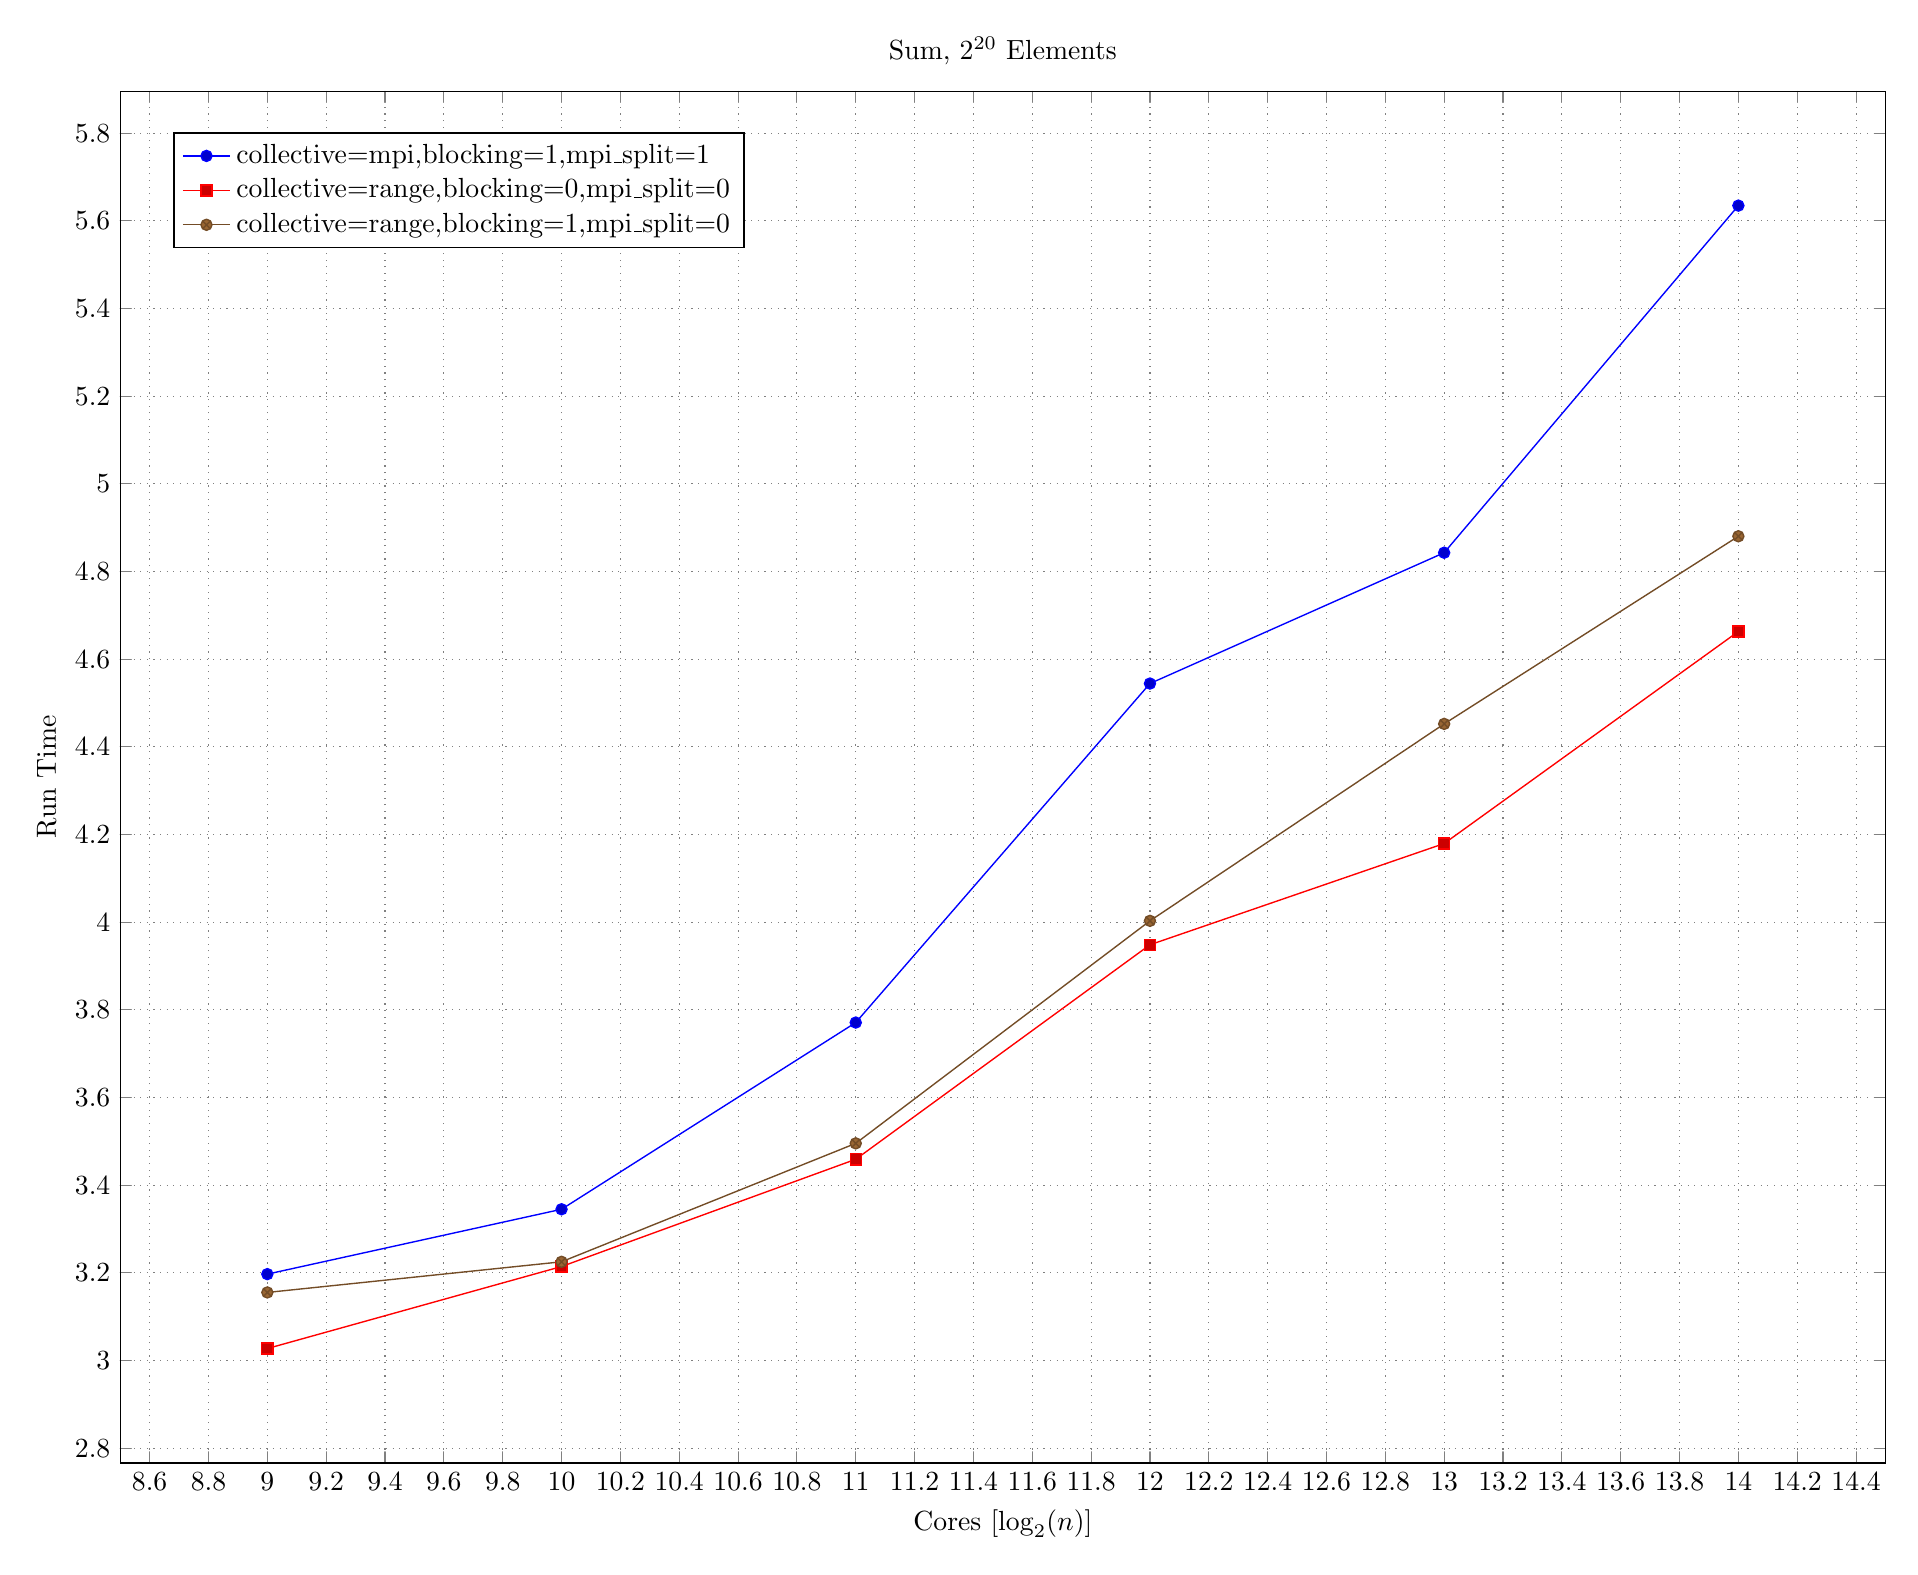
\begin{tikzpicture}
  \begin{axis}[
    title={Sum, $2^{20}$ Elements},
    xlabel={Cores [$\log_2(n)$]},
    ylabel={Run Time},
    ]   
	%% MULTIPLOT(collective, blocking, mpi_split) SELECT LOG(2,size) AS x, MEDIAN(sum) as y, MULTIPLOT
	%% FROM ResultsQS
	%% WHERE elements=POWER(2,20) AND (blocking=1 OR mpi_split=0)
	%% GROUP BY MULTIPLOT, x  ORDER BY MULTIPLOT, x
 \addplot coordinates { (9.0,3.197115) (10.0,3.34508) (11.0,3.77105) (12.0,4.5445) (13.0,4.84298) (14.0,5.63485) };
 \addlegendentry{collective=mpi,blocking=1,mpi\_split=1};
 \addplot coordinates { (9.0,3.02732) (10.0,3.21445) (11.0,3.45912) (12.0,3.94849) (13.0,4.1795) (14.0,4.66324) };
 \addlegendentry{collective=range,blocking=0,mpi\_split=0};
 \addplot coordinates { (9.0,3.15532) (10.0,3.22524) (11.0,3.49545) (12.0,4.00308) (13.0,4.45242) (14.0,4.88048) };
 \addlegendentry{collective=range,blocking=1,mpi\_split=0};


  \end{axis}
\end{tikzpicture}
\newpage


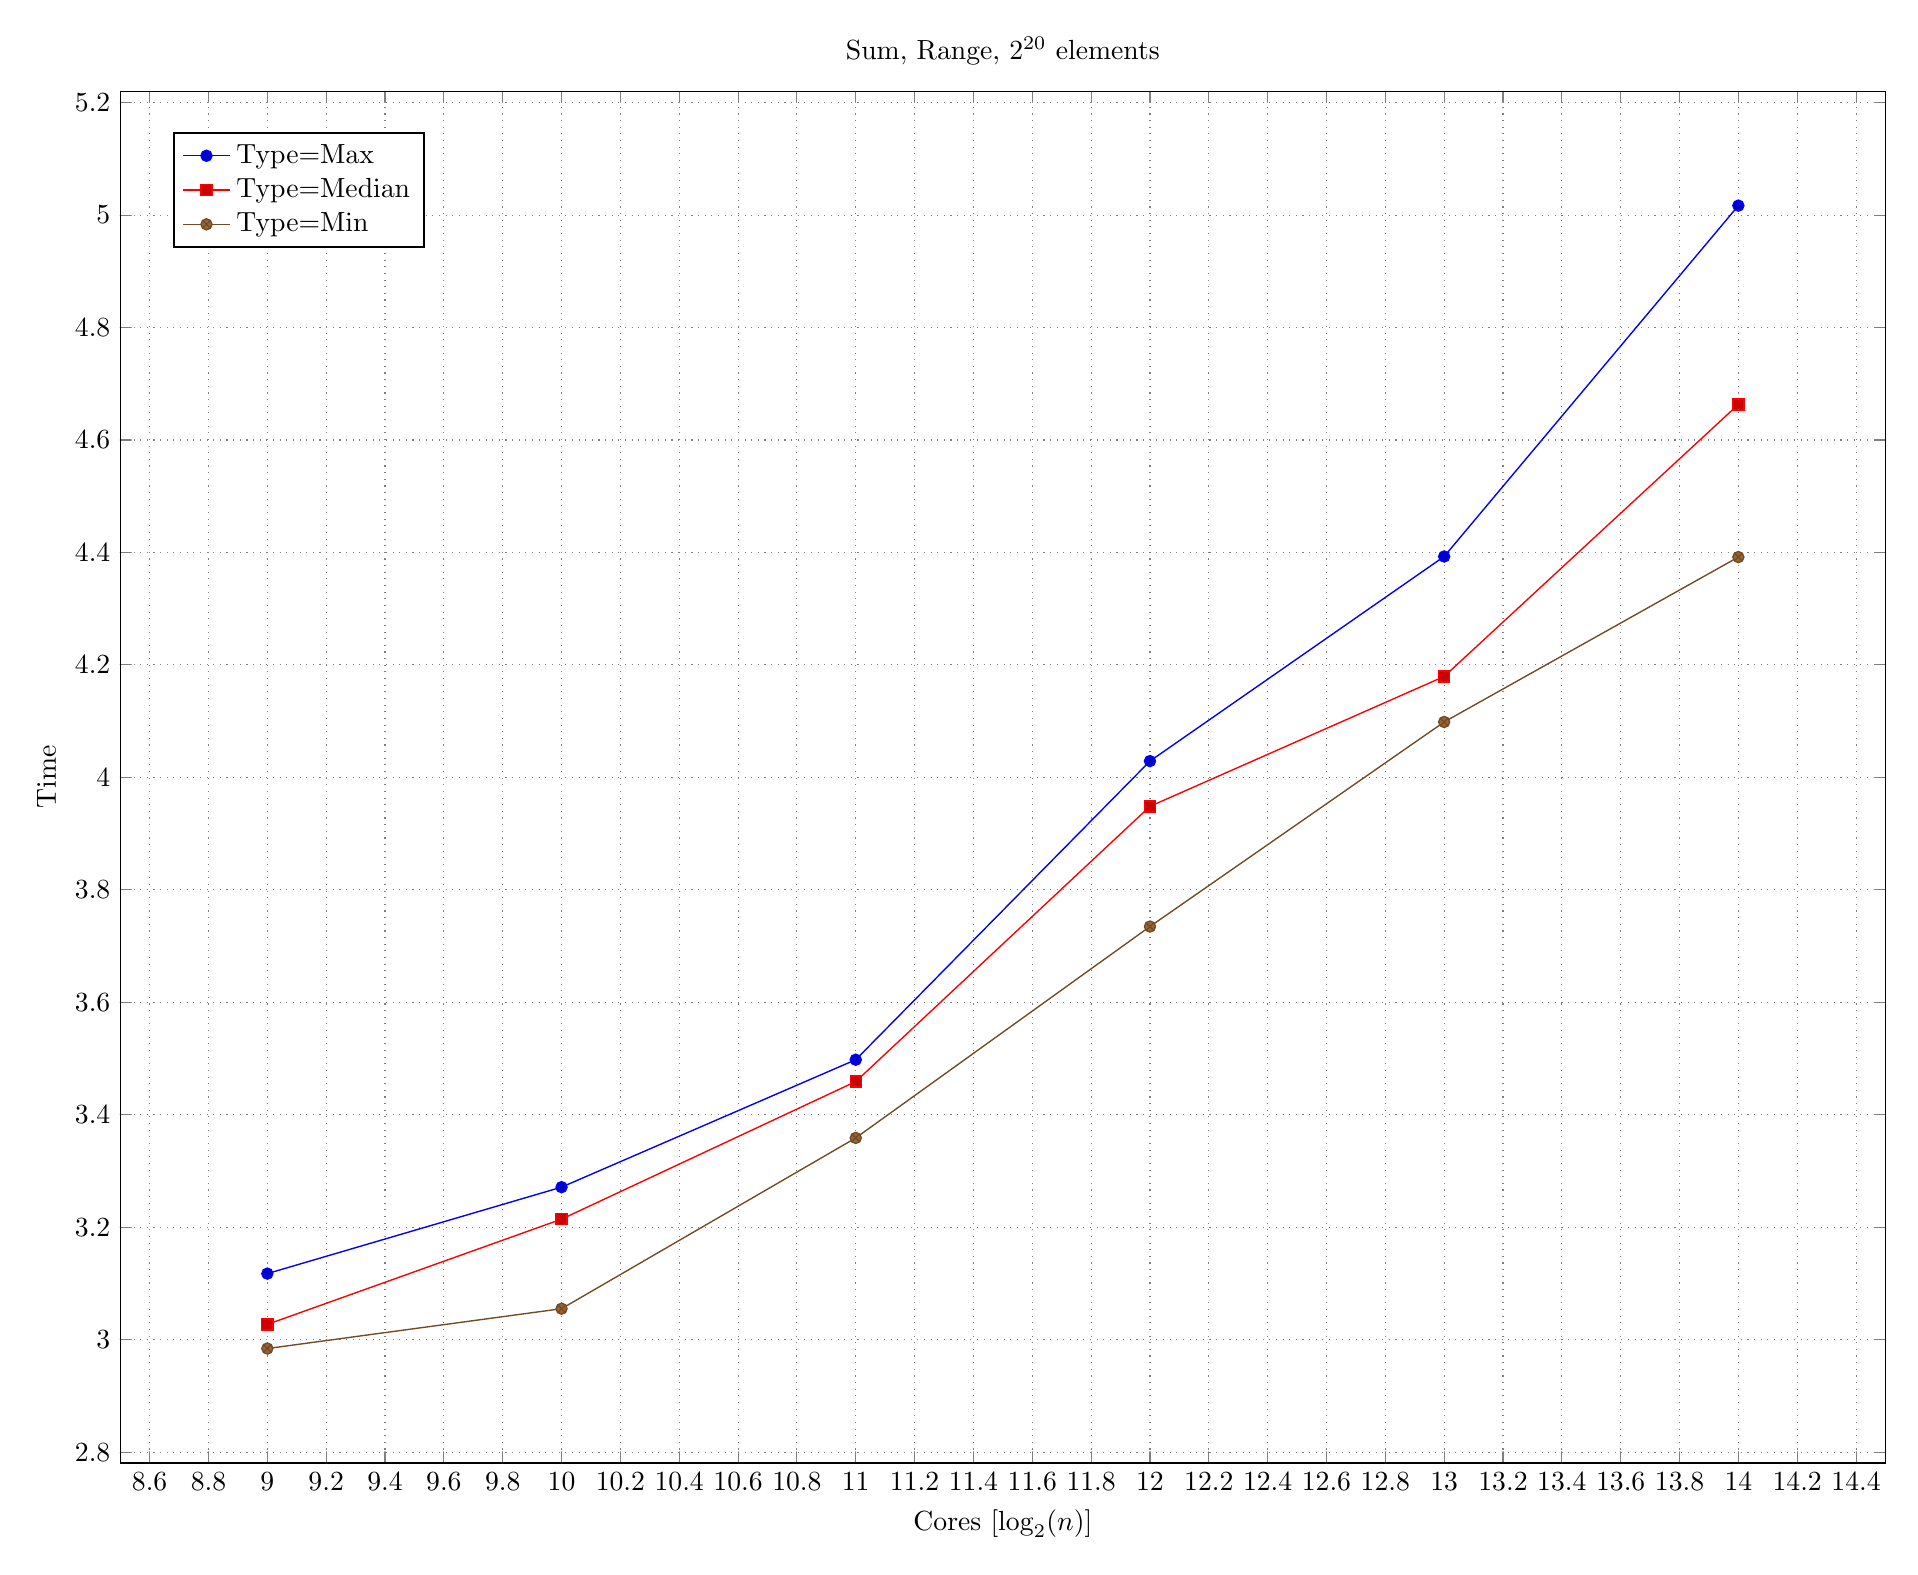
\begin{tikzpicture}
\begin{axis}[
title={Sum, Range, $2^{20}$ elements},
xlabel={Cores [$\log_2(n)$]},
ylabel={Time},
]   
%% MULTIPLOT(Type) SELECT elements, collective, blocking, mpi_split, LOG(2,size) AS x, Time as y, MULTIPLOT FROM (    
%% SELECT elements, size, MIN(sum) as Time, 'Min' as Type, collective, blocking, mpi_split
%% FROM ResultsQS
%% GROUP BY elements, size, collective, blocking, mpi_split
%% UNION ALL
%% SELECT elements, size, MEDIAN(sum) as Time, 'Median' as Type, collective, blocking, mpi_split
%% FROM ResultsQS
%% GROUP BY elements, size, collective, blocking, mpi_split
%% UNION ALL
%% SELECT elements, size, MAX(sum) as Time, 'Max' as Type, collective, blocking, mpi_split
%% FROM ResultsQS
%% GROUP BY elements, size, collective, blocking, mpi_split
%% ) a
%% WHERE elements=POWER(2,20) AND collective="range" AND blocking=0 AND mpi_split=0
%% GROUP BY MULTIPLOT, x  ORDER BY MULTIPLOT, x
\addplot coordinates { (9.0,3.11764) (10.0,3.27136) (11.0,3.49799) (12.0,4.029) (13.0,4.39285) (14.0,5.0168) };
\addlegendentry{Type=Max};
\addplot coordinates { (9.0,3.02732) (10.0,3.21445) (11.0,3.45912) (12.0,3.94849) (13.0,4.1795) (14.0,4.66324) };
\addlegendentry{Type=Median};
\addplot coordinates { (9.0,2.98436) (10.0,3.05521) (11.0,3.35889) (12.0,3.73481) (13.0,4.09857) (14.0,4.39182) };
\addlegendentry{Type=Min};
\end{axis}
\end{tikzpicture}
\newpage

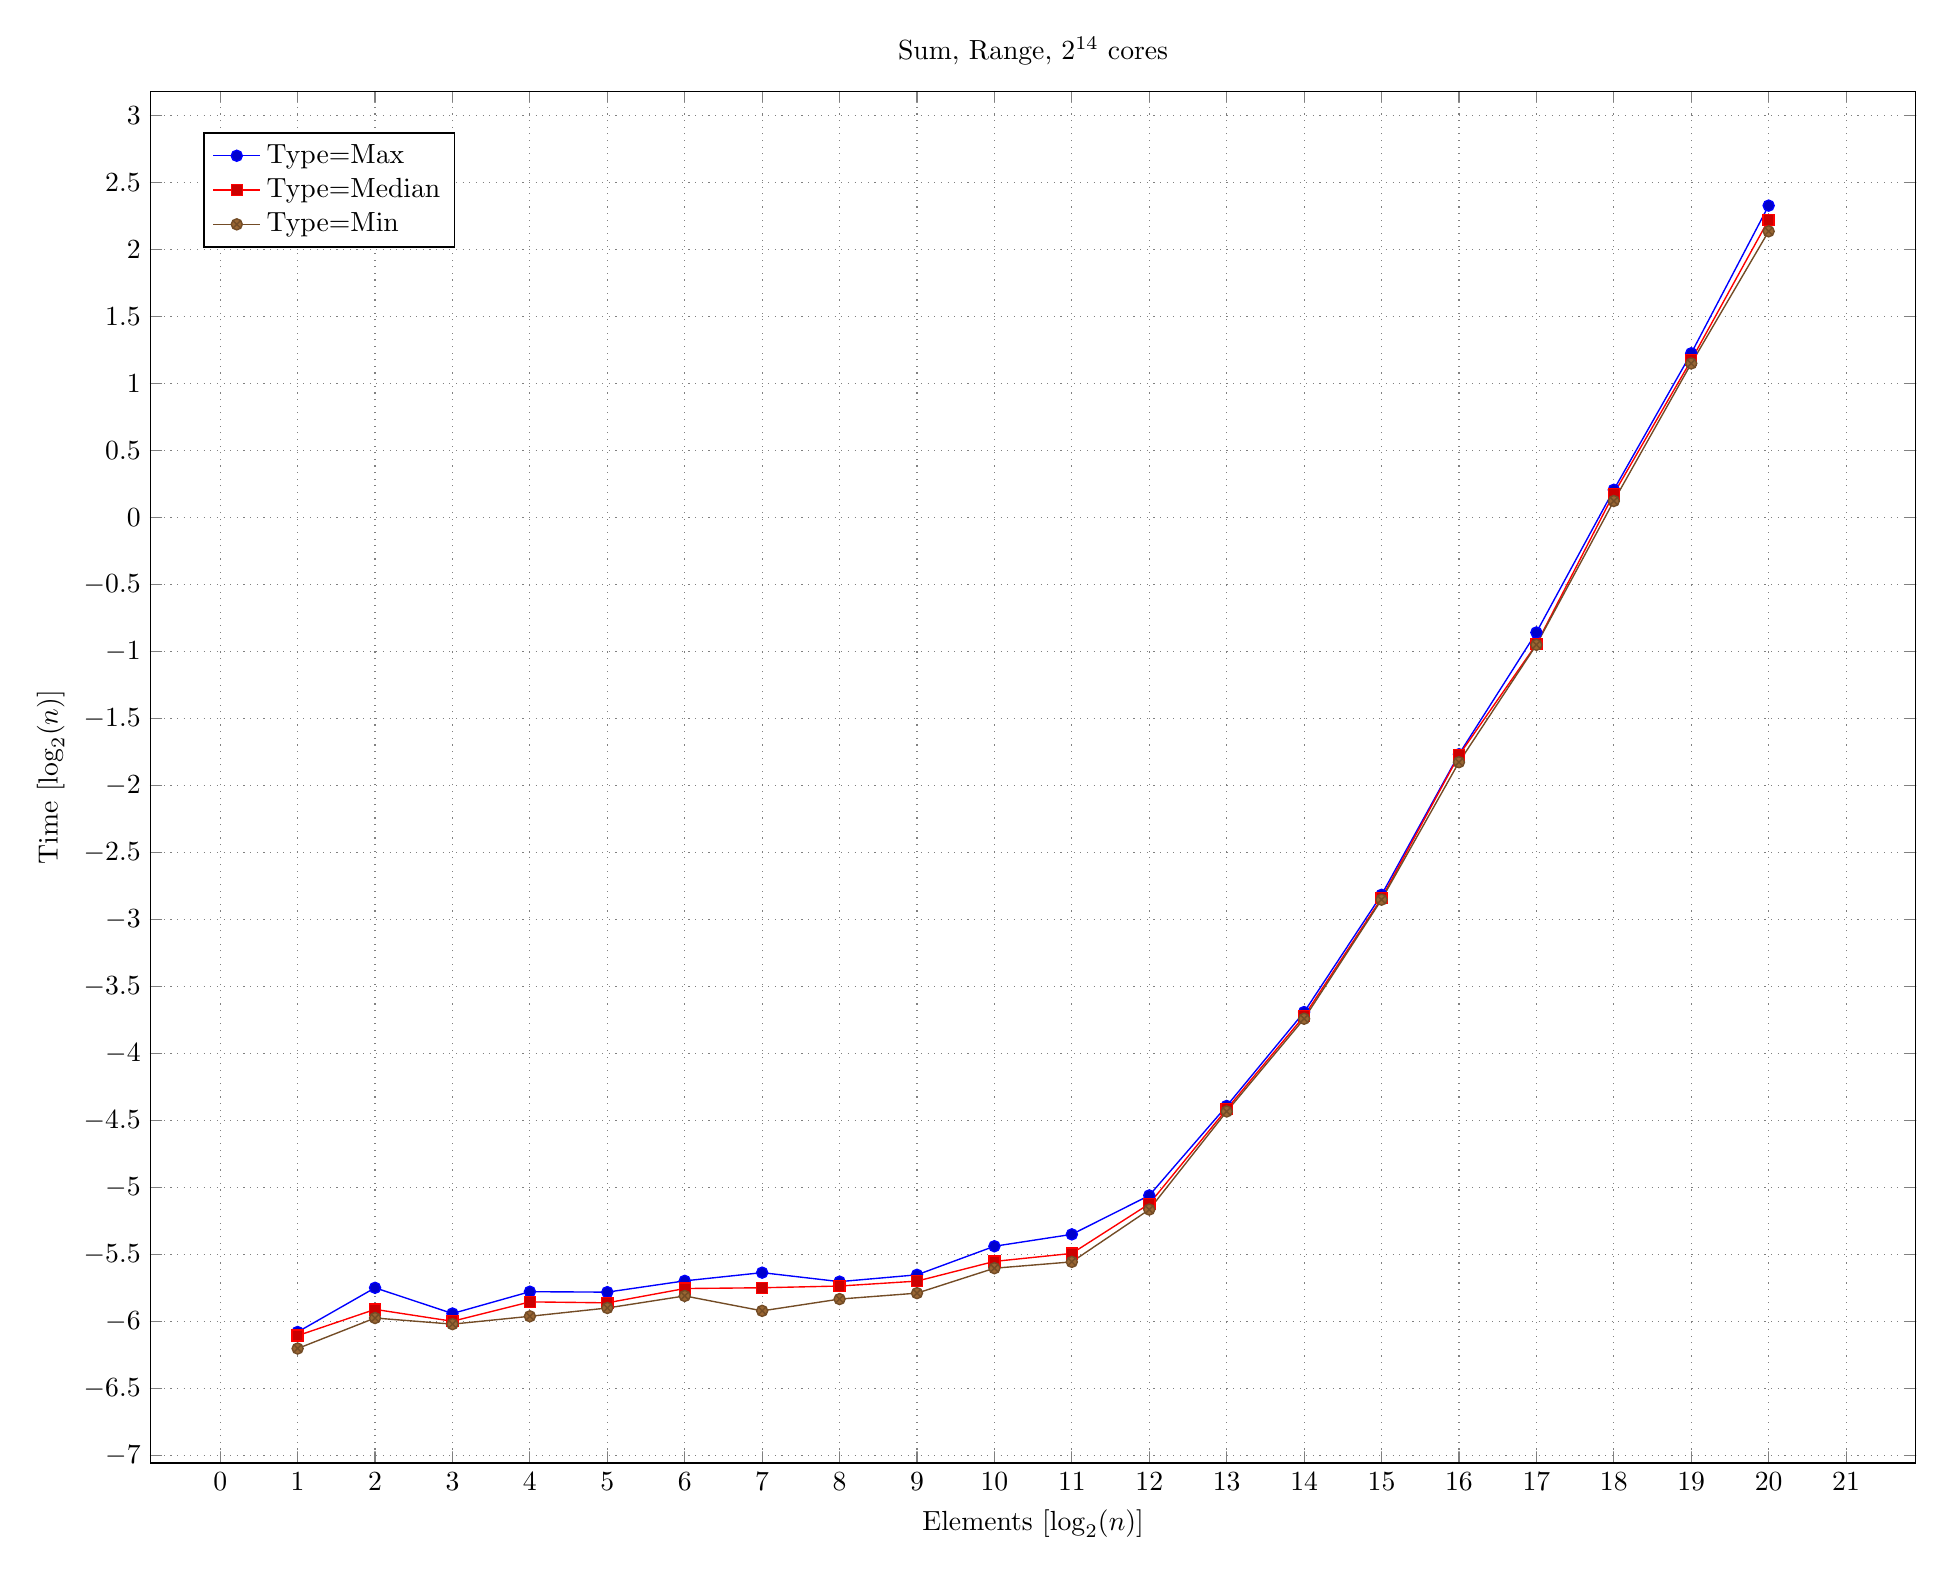
\begin{tikzpicture}
\begin{axis}[
title={Sum, Range, $2^{14}$ cores},
xlabel={Elements [$\log_2(n)$]},
ylabel={Time [$\log_2(n)$]},
]   
%% MULTIPLOT(Type) SELECT size, collective, blocking, mpi_split, LOG(2,elements) AS x, LOG(2,Time) as y, MULTIPLOT FROM (    
%% SELECT elements, size, MIN(sum) as Time, 'Min' as Type, collective, blocking, mpi_split
%% FROM ResultsQS
%% GROUP BY elements, size, collective, blocking, mpi_split
%% UNION ALL
%% SELECT elements, size, MEDIAN(sum) as Time, 'Median' as Type, collective, blocking, mpi_split
%% FROM ResultsQS
%% GROUP BY elements, size, collective, blocking, mpi_split
%% UNION ALL
%% SELECT elements, size, MAX(sum) as Time, 'Max' as Type, collective, blocking, mpi_split
%% FROM ResultsQS
%% GROUP BY elements, size, collective, blocking, mpi_split
%% ) a
%% WHERE size=16384 AND collective="range" AND blocking=0 AND mpi_split=0
%% GROUP BY MULTIPLOT, x  ORDER BY MULTIPLOT, x
\addplot coordinates { (1.0,-6.08003) (2.0,-5.7503) (3.0,-5.94206) (4.0,-5.77924) (5.0,-5.78258) (6.0,-5.69839) (7.0,-5.63714) (8.0,-5.70422) (9.0,-5.65335) (10.0,-5.44009) (11.0,-5.3514) (12.0,-5.06098) (13.0,-4.39301) (14.0,-3.69228) (15.0,-2.8172) (16.0,-1.76799) (17.0,-0.859145) (18.0,0.205843) (19.0,1.22463) (20.0,2.32677) };
\addlegendentry{Type=Max};
\addplot coordinates { (1.0,-6.10721) (2.0,-5.9113) (3.0,-6.00003) (4.0,-5.85525) (5.0,-5.86239) (6.0,-5.75577) (7.0,-5.74991) (8.0,-5.73707) (9.0,-5.70031) (10.0,-5.55325) (11.0,-5.49366) (12.0,-5.12376) (13.0,-4.41677) (14.0,-3.7221) (15.0,-2.84255) (16.0,-1.77549) (17.0,-0.946875) (18.0,0.176246) (19.0,1.17313) (20.0,2.22133) };
\addlegendentry{Type=Median};
\addplot coordinates { (1.0,-6.20356) (2.0,-5.97579) (3.0,-6.02147) (4.0,-5.96286) (5.0,-5.90094) (6.0,-5.81096) (7.0,-5.92231) (8.0,-5.83439) (9.0,-5.79008) (10.0,-5.60407) (11.0,-5.55669) (12.0,-5.16629) (13.0,-4.43418) (14.0,-3.74216) (15.0,-2.85339) (16.0,-1.82746) (17.0,-0.951382) (18.0,0.122076) (19.0,1.14843) (20.0,2.13482) };
\addlegendentry{Type=Min};
\end{axis}
\end{tikzpicture}
\newpage

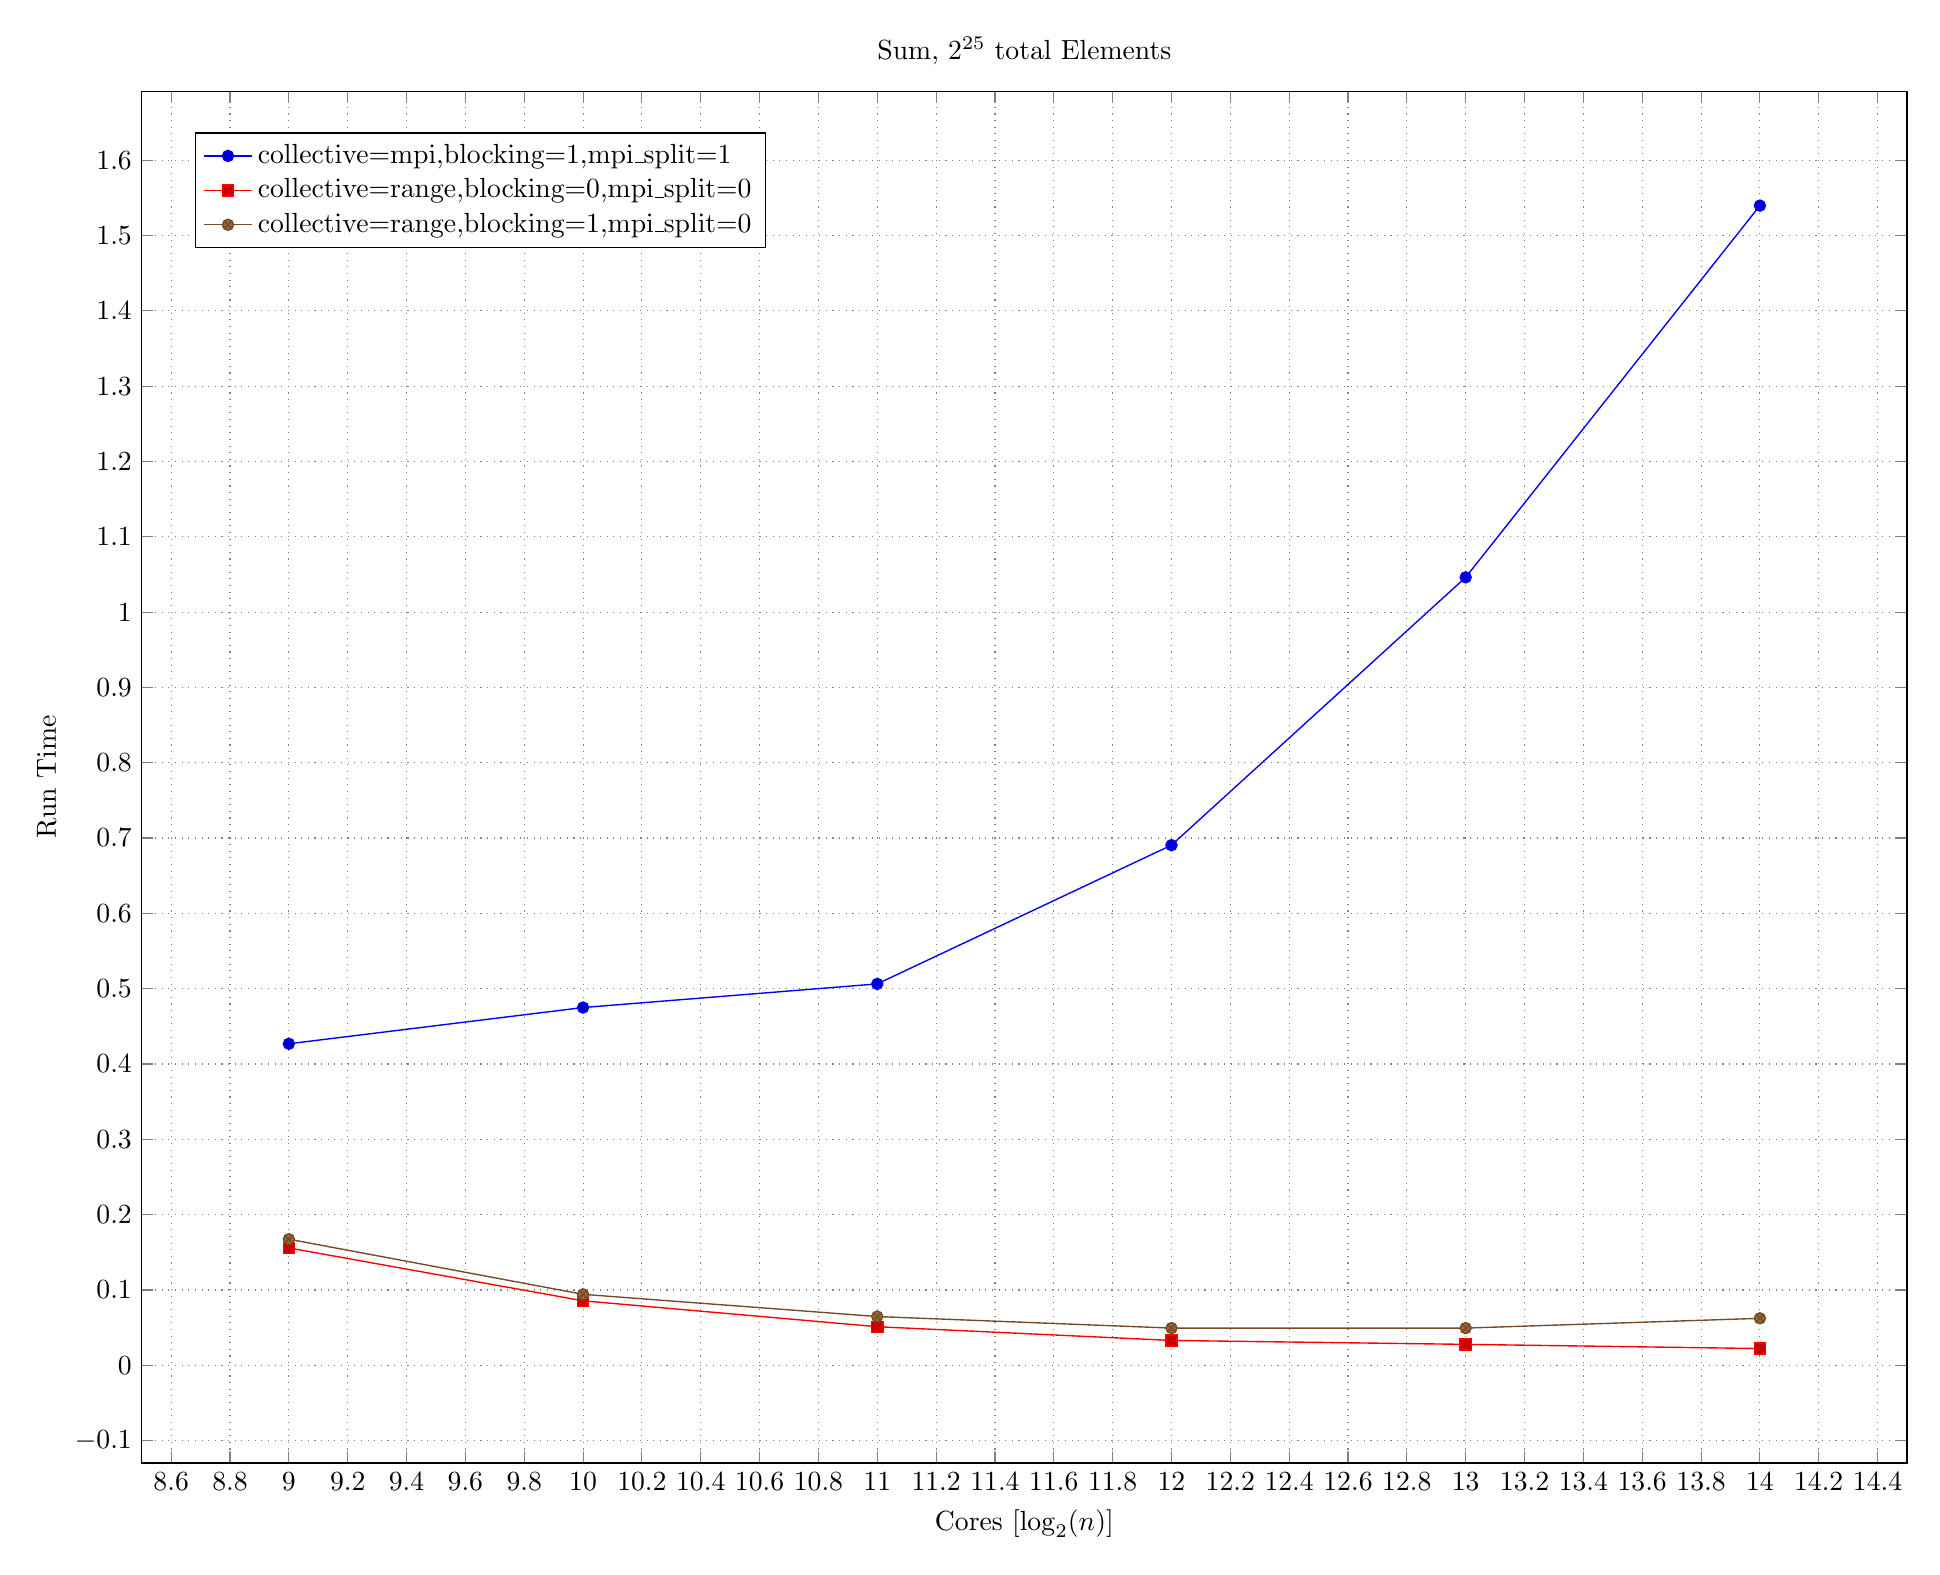
\begin{tikzpicture}
  \begin{axis}[
    title={Sum, $2^{25}$ total Elements},
    xlabel={Cores [$\log_2(n)$]},
    ylabel={Run Time},
    ]   
	%% MULTIPLOT(collective, blocking, mpi_split) SELECT LOG(2,size) AS x, MEDIAN(sum) as y, MULTIPLOT
	%% FROM ResultsQS
	%% WHERE elements*size=POWER(2,25) AND (blocking=1 OR mpi_split=0)
	%% GROUP BY MULTIPLOT, x  ORDER BY MULTIPLOT, x
 \addplot coordinates { (9.0,0.426851) (10.0,0.474958) (11.0,0.506346) (12.0,0.690566) (13.0,1.04616) (14.0,1.53968) };
 \addlegendentry{collective=mpi,blocking=1,mpi\_split=1};
 \addplot coordinates { (9.0,0.155784) (10.0,0.0855979) (11.0,0.0511719) (12.0,0.0329661) (13.0,0.0277636) (14.0,0.0221944) };
 \addlegendentry{collective=range,blocking=0,mpi\_split=0};
 \addplot coordinates { (9.0,0.167381) (10.0,0.0941817) (11.0,0.0646971) (12.0,0.0493551) (13.0,0.0493706) (14.0,0.0623134) };
 \addlegendentry{collective=range,blocking=1,mpi\_split=0};


  \end{axis}
\end{tikzpicture}
\newpage

\begin{tikzpicture}
\begin{axis}[
title={Depth},
xlabel={Cores [$\log_2(n)$]},
ylabel={Depth},
]   
%% MULTIPLOT(Type) SELECT LOG(2,size) AS x, Time as y, MULTIPLOT FROM (    
%% SELECT elements, size, MEDIAN(depth) as Time, 'Median' as Type
%% FROM ResultsQS
%% WHERE elements>POWER(2,10)
%% GROUP BY size
%% UNION ALL
%% SELECT elements, size, MIN(depth) as Time, 'Min' as Type
%% FROM ResultsQS
%% WHERE elements>POWER(2,10)
%% GROUP BY size
%% UNION ALL
%% SELECT elements, size, MAX(depth) as Time, 'Max' as Type
%% FROM ResultsQS
%% WHERE elements>POWER(2,10)
%% GROUP BY size
%% ) a
%% WHERE 1
%% GROUP BY MULTIPLOT, x  ORDER BY MULTIPLOT, x
\addplot coordinates { (9.0,21) (10.0,26) (11.0,27) (12.0,29) (13.0,31) (14.0,33) };
\addlegendentry{Type=Max};
\addplot coordinates { (9.0,17) (10.0,19) (11.0,21.5) (12.0,23) (13.0,26) (14.0,28) };
\addlegendentry{Type=Median};
\addplot coordinates { (9.0,15) (10.0,17) (11.0,19) (12.0,21) (13.0,24) (14.0,26) };
\addlegendentry{Type=Min};


\end{axis}
\end{tikzpicture}
\newpage

%\begin{tikzpicture}
%\begin{axis}[
%title={Pivot, $2^{20}$ elements},
%xlabel={Cores [$\log_2(n)$]},
%ylabel={Run Time},
%]   
% %% MULTIPLOT(Type) SELECT elements, LOG(2,size) AS x, Time as y, MULTIPLOT FROM (    
% %% SELECT elements, size, MEDIAN(pivot) as Time, 'Range' as Type
% %% FROM ResultsQS
% %% WHERE collective="range" AND blocking=0 AND mpi_split=0
% %% GROUP BY size, elements
% %% UNION ALL
% %% SELECT elements, size, MEDIAN(pivot) as Time, 'Range blocking' as Type
% %% FROM ResultsQS
% %% WHERE collective="range" AND blocking=1 AND mpi_split=0
% %% GROUP BY size, elements
% %% UNION ALL
% %% SELECT elements, size, MEDIAN(pivot) as Time, 'Range mpi_split' as Type
% %% FROM ResultsQS
% %% WHERE collective="range" AND blocking=0 AND mpi_split=1
% %% GROUP BY size, elements
% %% UNION ALL
% %% SELECT elements, size, MEDIAN(pivot) as Time, 'MPI blocking' as Type
% %% FROM ResultsQS
% %% WHERE collective="mpi" AND blocking=1 AND mpi_split=1
% %% GROUP BY size, elements
% %% ) a
% %% WHERE elements=POWER(2,20)
% %% GROUP BY MULTIPLOT, x  ORDER BY MULTIPLOT, x
%\addplot coordinates { (9.0,0.0774949) (10.0,0.0483513) (12.0,0.0597702) (13.0,0.0625685) };
%\addlegendentry{Type=MPI blocking};
%\addplot coordinates { (9.0,0.125294) (10.0,0.123921) (12.0,0.146194) (13.0,0.151579) };
%\addlegendentry{Type=Range};
%\addplot coordinates { (9.0,0.223502) (10.0,0.195748) (12.0,0.291215) (13.0,0.398244) };
%\addlegendentry{Type=Range blocking};
%\addplot coordinates { (9.0,0.0172105) (10.0,0.0280767) (12.0,0.0579143) (13.0,0.0791711) };
%\addlegendentry{Type=Range mpi\_split};
%
%
%\end{axis}
%\end{tikzpicture}
%\newpage
%
%\begin{tikzpicture}
%\begin{axis}[
%title={Prefix sum, $2^{20}$ elements},
%xlabel={Cores [$\log_2(n)$]},
%ylabel={Run Time},
%]   
% %% MULTIPLOT(Type) SELECT elements, LOG(2,size) AS x, Time as y, MULTIPLOT FROM (    
% %% SELECT elements, size, MEDIAN(calculate) as Time, 'Range' as Type
% %% FROM ResultsQS
% %% WHERE collective="range" AND blocking=0 AND mpi_split=0
% %% GROUP BY size, elements
% %% UNION ALL
% %% SELECT elements, size, MEDIAN(calculate) as Time, 'Range blocking' as Type
% %% FROM ResultsQS
% %% WHERE collective="range" AND blocking=1 AND mpi_split=0
% %% GROUP BY size, elements
% %% UNION ALL
% %% SELECT elements, size, MEDIAN(calculate) as Time, 'Range mpi_split' as Type
% %% FROM ResultsQS
% %% WHERE collective="range" AND blocking=0 AND mpi_split=1
% %% GROUP BY size, elements
% %% UNION ALL
% %% SELECT elements, size, MEDIAN(calculate) as Time, 'MPI blocking' as Type
% %% FROM ResultsQS
% %% WHERE collective="mpi" AND blocking=1 AND mpi_split=1
% %% GROUP BY size, elements
% %% ) a
% %% WHERE elements=POWER(2,20)
% %% GROUP BY MULTIPLOT, x  ORDER BY MULTIPLOT, x
%\addplot coordinates { (9.0,0.0544872) (10.0,0.054643) (12.0,0.0933107) (13.0,0.103632) };
%\addlegendentry{Type=MPI blocking};
%\addplot coordinates { (9.0,0.0733838) (10.0,0.0860003) (12.0,0.134109) (13.0,0.145614) };
%\addlegendentry{Type=Range};
%\addplot coordinates { (9.0,0.0567608) (10.0,0.0705758) (12.0,0.0870146) (13.0,0.132569) };
%\addlegendentry{Type=Range blocking};
%\addplot coordinates { (9.0,0.0537762) (10.0,0.0647017) (12.0,0.11611) (13.0,0.125948) };
%\addlegendentry{Type=Range mpi\_split};
%
%
%\end{axis}
%\end{tikzpicture}
%\newpage

\end{center}

\end{document}

%%%%%%%%%%%%%%%%%%%%%%%%%%%%%%%%%%%%%%%%%%%%%%%%%%%%%%%%%%%%%%%%%%%%%%%%%%%%%%%%
